\documentclass[aspectratio=169]{beamer}

% Professional, Minimalist, Academic & Corporate Theme
\usepackage{tikz}
\usepackage{xcolor}
\usepackage{listings}
\usepackage{booktabs}
\usepackage{graphicx}
\usepackage{array}

% Custom elegant colors
\definecolor{AmritaMaroon}{HTML}{800000}
\definecolor{NavyBlue}{HTML}{002855}
\definecolor{LightGray}{HTML}{F3F4F6}
\definecolor{DarkGray}{HTML}{374151}
\definecolor{EmeraldGreen}{HTML}{047857}
\definecolor{BorderGray}{HTML}{D1D5DB}

% Code Listing Style
\lstdefinestyle{mystyle}{
    backgroundcolor=\color{LightGray},   
    commentstyle=\color{AmritaMaroon},
    keywordstyle=\color{NavyBlue}\bfseries,
    numberstyle=\tiny\color{DarkGray},
    stringstyle=\color{AmritaMaroon},
    basicstyle=\ttfamily\fontsize{5.2}{6.4}\selectfont\color{DarkGray},
    breaklines=true,                 
    captionpos=b,                    
    keepspaces=true,                 
    showspaces=false,                
    showstringspaces=false,
    showtabs=false,                  
    tabsize=2
}
\lstset{style=mystyle}

% Terminal Output Listing Style
\lstdefinestyle{termstyle}{
    backgroundcolor=\color{LightGray},
    basicstyle=\ttfamily\fontsize{5.0}{6.2}\selectfont\color{DarkGray},
    breaklines=true,
    keepspaces=true,
    showspaces=false,
    showstringspaces=false,
    tabsize=2
}

% Beamer Theme Settings
\mode<presentation>{
    \usetheme{default}
    \setbeamercolor{background canvas}{bg=white}
    \setbeamercolor{normal text}{fg=DarkGray}
    \setbeamercolor{title}{fg=NavyBlue}
    \setbeamercolor{subtitle}{fg=AmritaMaroon}
    \setbeamercolor{frametitle}{fg=NavyBlue, bg=white}
    \setbeamercolor{structure}{fg=NavyBlue}
    \setbeamercolor{itemize item}{fg=AmritaMaroon}
    \setbeamercolor{itemize subitem}{fg=NavyBlue}
    \setbeamercolor{block title}{fg=white, bg=NavyBlue}
    \setbeamercolor{block body}{bg=LightGray}
    
    \setbeamerfont{title}{size=\huge, series=\bfseries}
    \setbeamerfont{subtitle}{size=\Large, series=\bfseries}
    \setbeamerfont{frametitle}{size=\normalsize, series=\bfseries}
    \setbeamerfont{author}{size=\normalsize}
    
    \setbeamertemplate{navigation symbols}{}
    
    \setbeamersize{text margin left=0.7cm, text margin right=0.7cm}
    
    \setbeamertemplate{frametitle}{%
        \vspace{0.15cm}%
        \noindent\usebeamerfont{frametitle}\insertframetitle\par%
        \vspace{0.04cm}%
        {\color{AmritaMaroon}\rule{\textwidth}{1pt}}\par%
        \vspace{0.08cm}%
    }
    
    \setbeamertemplate{footline}{%
        \leavevmode%
        \vbox{%
            {\color{BorderGray}\rule{\paperwidth}{0.4pt}}\vskip2pt%
            \hbox{%
                \begin{beamercolorbox}[wd=.333333\paperwidth,ht=2.0ex,dp=0.8ex,left]{author in head/foot}%
                    \hspace*{2ex}\tiny\textcolor{DarkGray}{\textbf{Amrita Vishwa Vidyapeetham}}%
                \end{beamercolorbox}%
                \begin{beamercolorbox}[wd=.333333\paperwidth,ht=2.0ex,dp=0.8ex,center]{title in head/foot}%
                    \tiny\textcolor{DarkGray}{\textbf{23CSE352: Big Data Analytics (Review 2)}}%
                \end{beamercolorbox}%
                \begin{beamercolorbox}[wd=.333333\paperwidth,ht=2.0ex,dp=0.8ex,right]{date in head/foot}%
                    \tiny\textcolor{AmritaMaroon}{\textbf{\insertframenumber{} / \inserttotalframenumber}}\hspace*{2ex}%
                \end{beamercolorbox}%
            }%
            \vskip2pt%
        }%
    }
}

\title{Big Data Analytics of Crime Patterns}
\subtitle{Project Review 2: Distributed Real-Time Serving using Apache HBase}
\author{\textbf{Team Members:}\\[0.15cm] Sheela Akshar Sakhi (\texttt{CB.SC.U4CSE23547}) \quad \& \quad Nishanth S Gowda (\texttt{CB.SC.U4CSE23538})}
\institute{Department of Computer Science and Engineering\\Amrita Vishwa Vidyapeetham}
\date{\today}

\begin{document}

% ==========================================================================
% SLIDE 1: Title Page
% ==========================================================================
\begin{frame}[plain]
    \titlepage
\end{frame}

% ==========================================================================
% SLIDE 2: Application Introduction, Problem Statement & Paradigm Shift
% ==========================================================================
\begin{frame}{Application Introduction, Problem Statement \& Paradigm Shift}
    \begin{columns}[T]
        \begin{column}{0.48\textwidth}
            \textbf{\textcolor{NavyBlue}{Review 1 $\to$ Review 2 Paradigm Shift:}}
            \vspace{0.05cm}
            \begin{itemize}\footnotesize
                \setlength{\itemsep}{2pt}
                \item \textbf{Review 1 (Batch OLAP):} Hadoop MapReduce \& Hive -- high-latency batch aggregations; no random read/write access.
                \item \textbf{Review 2 (Real-Time NoSQL):} \textbf{Apache HBase} on HDFS -- sub-second point lookups (\texttt{GET}), selective column scans, and prefix filtering.
            \end{itemize}
            \vspace{0.08cm}
            \textbf{\textcolor{NavyBlue}{Operational Public Safety Domain:}}
            \begin{itemize}\footnotesize
                \setlength{\itemsep}{1pt}
                \item Rapid incident lookups for active 911 dispatches.
                \item Precinct-level crime monitoring and patrol deployment.
            \end{itemize}
        \end{column}
        \begin{column}{0.48\textwidth}
            \textbf{\textcolor{AmritaMaroon}{Core Challenges in Urban Policing:}}
            \vspace{0.05cm}
            \begin{itemize}\footnotesize
                \setlength{\itemsep}{1pt}
                \item Police departments generate tens of thousands of incident reports weekly with streaming updates.
                \item RDBMS systems suffer write contention and lock degradation under concurrent ingestion loads.
                \item HDFS batch files cannot provide sub-second point lookups for active investigations.
            \end{itemize}
            \vspace{0.06cm}
            \textbf{\textcolor{AmritaMaroon}{Why Apache HBase?}}
            \begin{itemize}\footnotesize
                \setlength{\itemsep}{1pt}
                \item Wide-column distributed NoSQL database natively on HDFS.
                \item Sub-5ms random read/write access to millions of records.
                \item Anti-hotspotting composite row key balances region servers.
            \end{itemize}
        \end{column}
    \end{columns}
\end{frame}

% ==========================================================================
% SLIDE 3: Real-World Dataset + Schema Mapping
% ==========================================================================
\begin{frame}{Step 2: Real-World Dataset (City of Chicago Crimes)}
    \begin{columns}[T]
        \begin{column}{0.42\textwidth}
            \textbf{\textcolor{NavyBlue}{Dataset Provenance \& Scale:}}
            \vspace{0.05cm}
            \begin{itemize}\footnotesize
                \setlength{\itemsep}{2pt}
                \item \textbf{Source:} Chicago Police Department (CLEAR system via Socrata Open Data API).
                \item \textbf{Scale:} 10,000+ authentic incident records with 22 attributes.
                \item \textbf{Provenance:} Official municipal government data -- \textbf{100\% real crime data}, strictly non-synthetic.
                \item \textbf{Attributes:} Case Number, Date, Block, IUCR Code, Primary Type, Description, Location, Arrest, Domestic, Beat, District, GPS Coordinates.
            \end{itemize}
        \end{column}
        \begin{column}{0.55\textwidth}
            \textbf{\textcolor{NavyBlue}{HBase Schema Mapping:}}
            \vspace{0.04cm}
            \begin{table}
                \centering
                \fontsize{5.2}{6.8}\selectfont
                \setlength{\tabcolsep}{2.5pt}
                \begin{tabular}{p{2.3cm}p{1.0cm}p{3.5cm}}
                    \toprule
                    \textbf{Attribute} & \textbf{Data Type} & \textbf{HBase Target Mapping} \\
                    \midrule
                    \texttt{id}, \texttt{district}, \texttt{primary\_type} & IDs & \textbf{Row Key:} \texttt{District\#CrimeType\#ID} \\
                    \texttt{case\_number}, \texttt{date}, \texttt{block} & Text & \textbf{CF:} \texttt{incident} (\texttt{VERSIONS => 3}) \\
                    \texttt{location\_desc}, \texttt{arrest}, \texttt{beat} & Bool/Code & \textbf{CF:} \texttt{details} (Administrative) \\
                    \texttt{latitude}, \texttt{longitude} & Float GPS & \textbf{CF:} \texttt{geo} (Spatial telemetry) \\
                    \bottomrule
                \end{tabular}
            \end{table}
            \vspace{0.04cm}
            \begin{itemize}\footnotesize
                \setlength{\itemsep}{1pt}
                \item Preprocessed to sanitize line breaks \& null values.
                \item Direct continuity with Review 1 crime dataset.
            \end{itemize}
        \end{column}
    \end{columns}
\end{frame}

% ==========================================================================
% SLIDE 4: System Architecture & Composite Row Key Design
% ==========================================================================
\begin{frame}{System Architecture \& Composite Row Key Design}
    \begin{columns}[T]
        \begin{column}{0.48\textwidth}
            \centering
            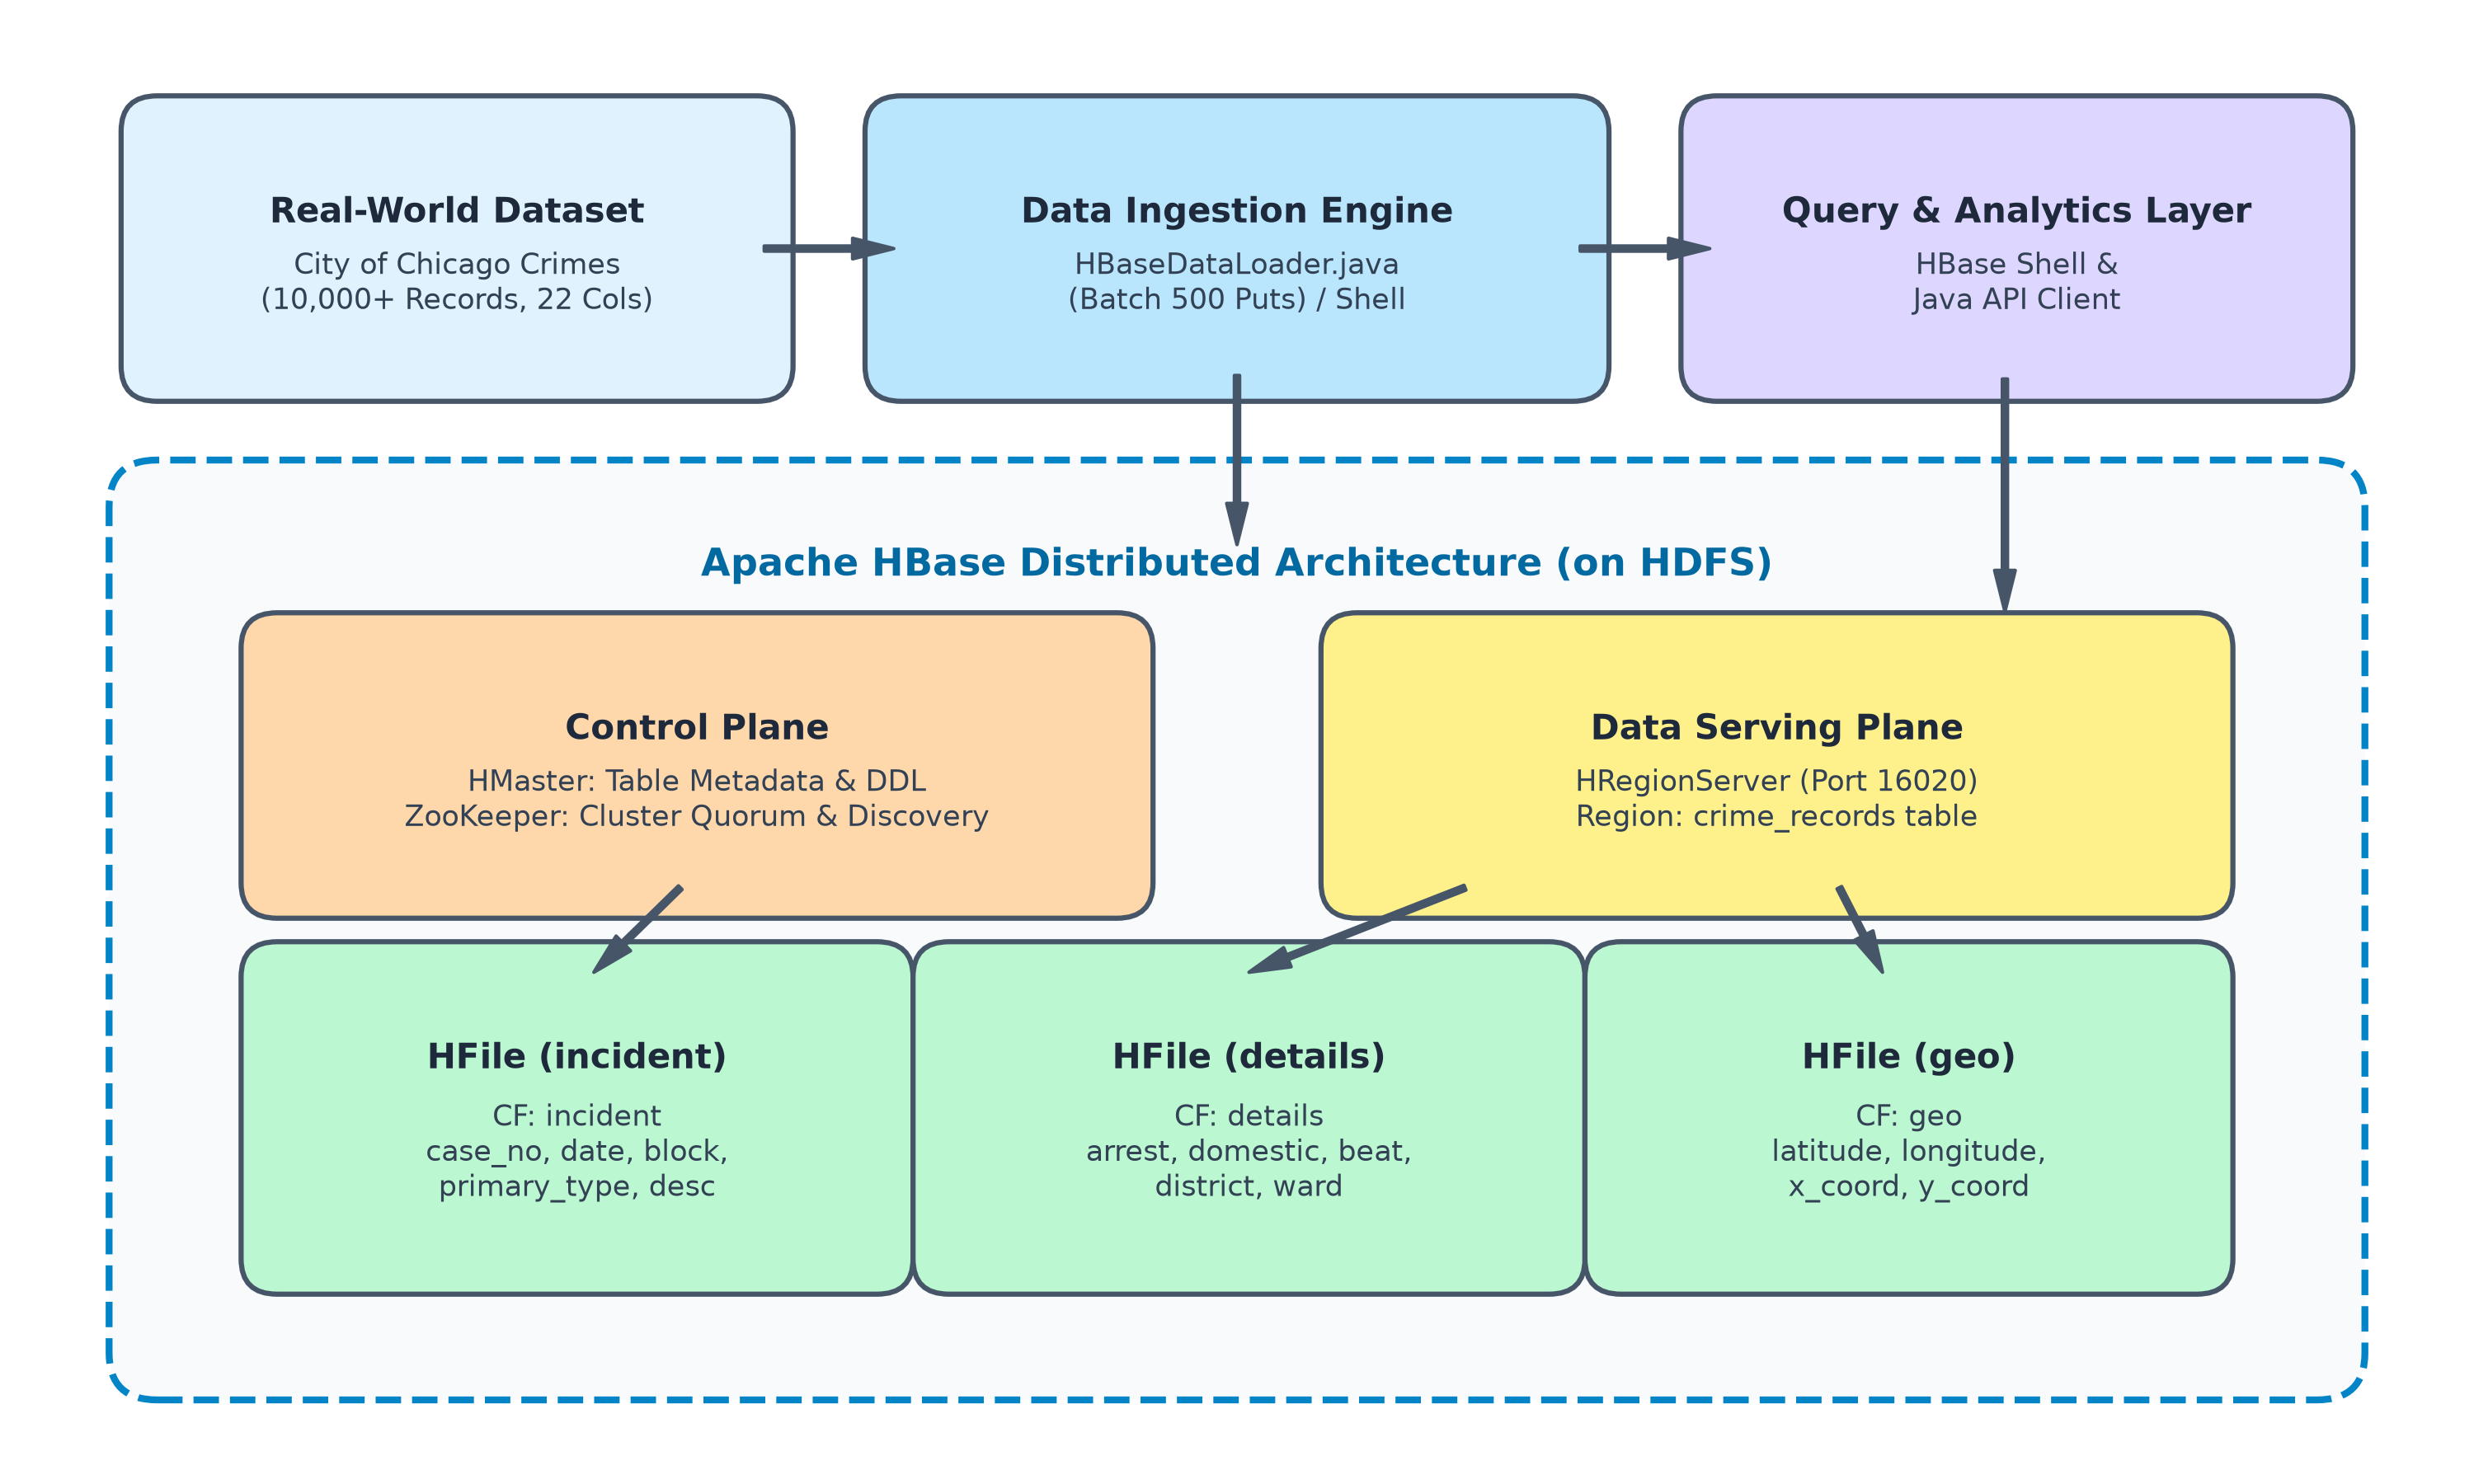
\includegraphics[height=3.4cm,keepaspectratio]{images/hbase_architecture.png}
            \vspace{0.04cm}
            \par{\tiny\textit{Figure 1: HBase Distributed Architecture on HDFS}}
            \begin{itemize}\scriptsize
                \setlength{\itemsep}{1pt}
                \item \textbf{HMaster \& ZooKeeper:} Cluster state, region balancing.
                \item \textbf{HRegionServers:} Host MemStore, WAL, and HFiles.
            \end{itemize}
        \end{column}
        \begin{column}{0.48\textwidth}
            \centering
            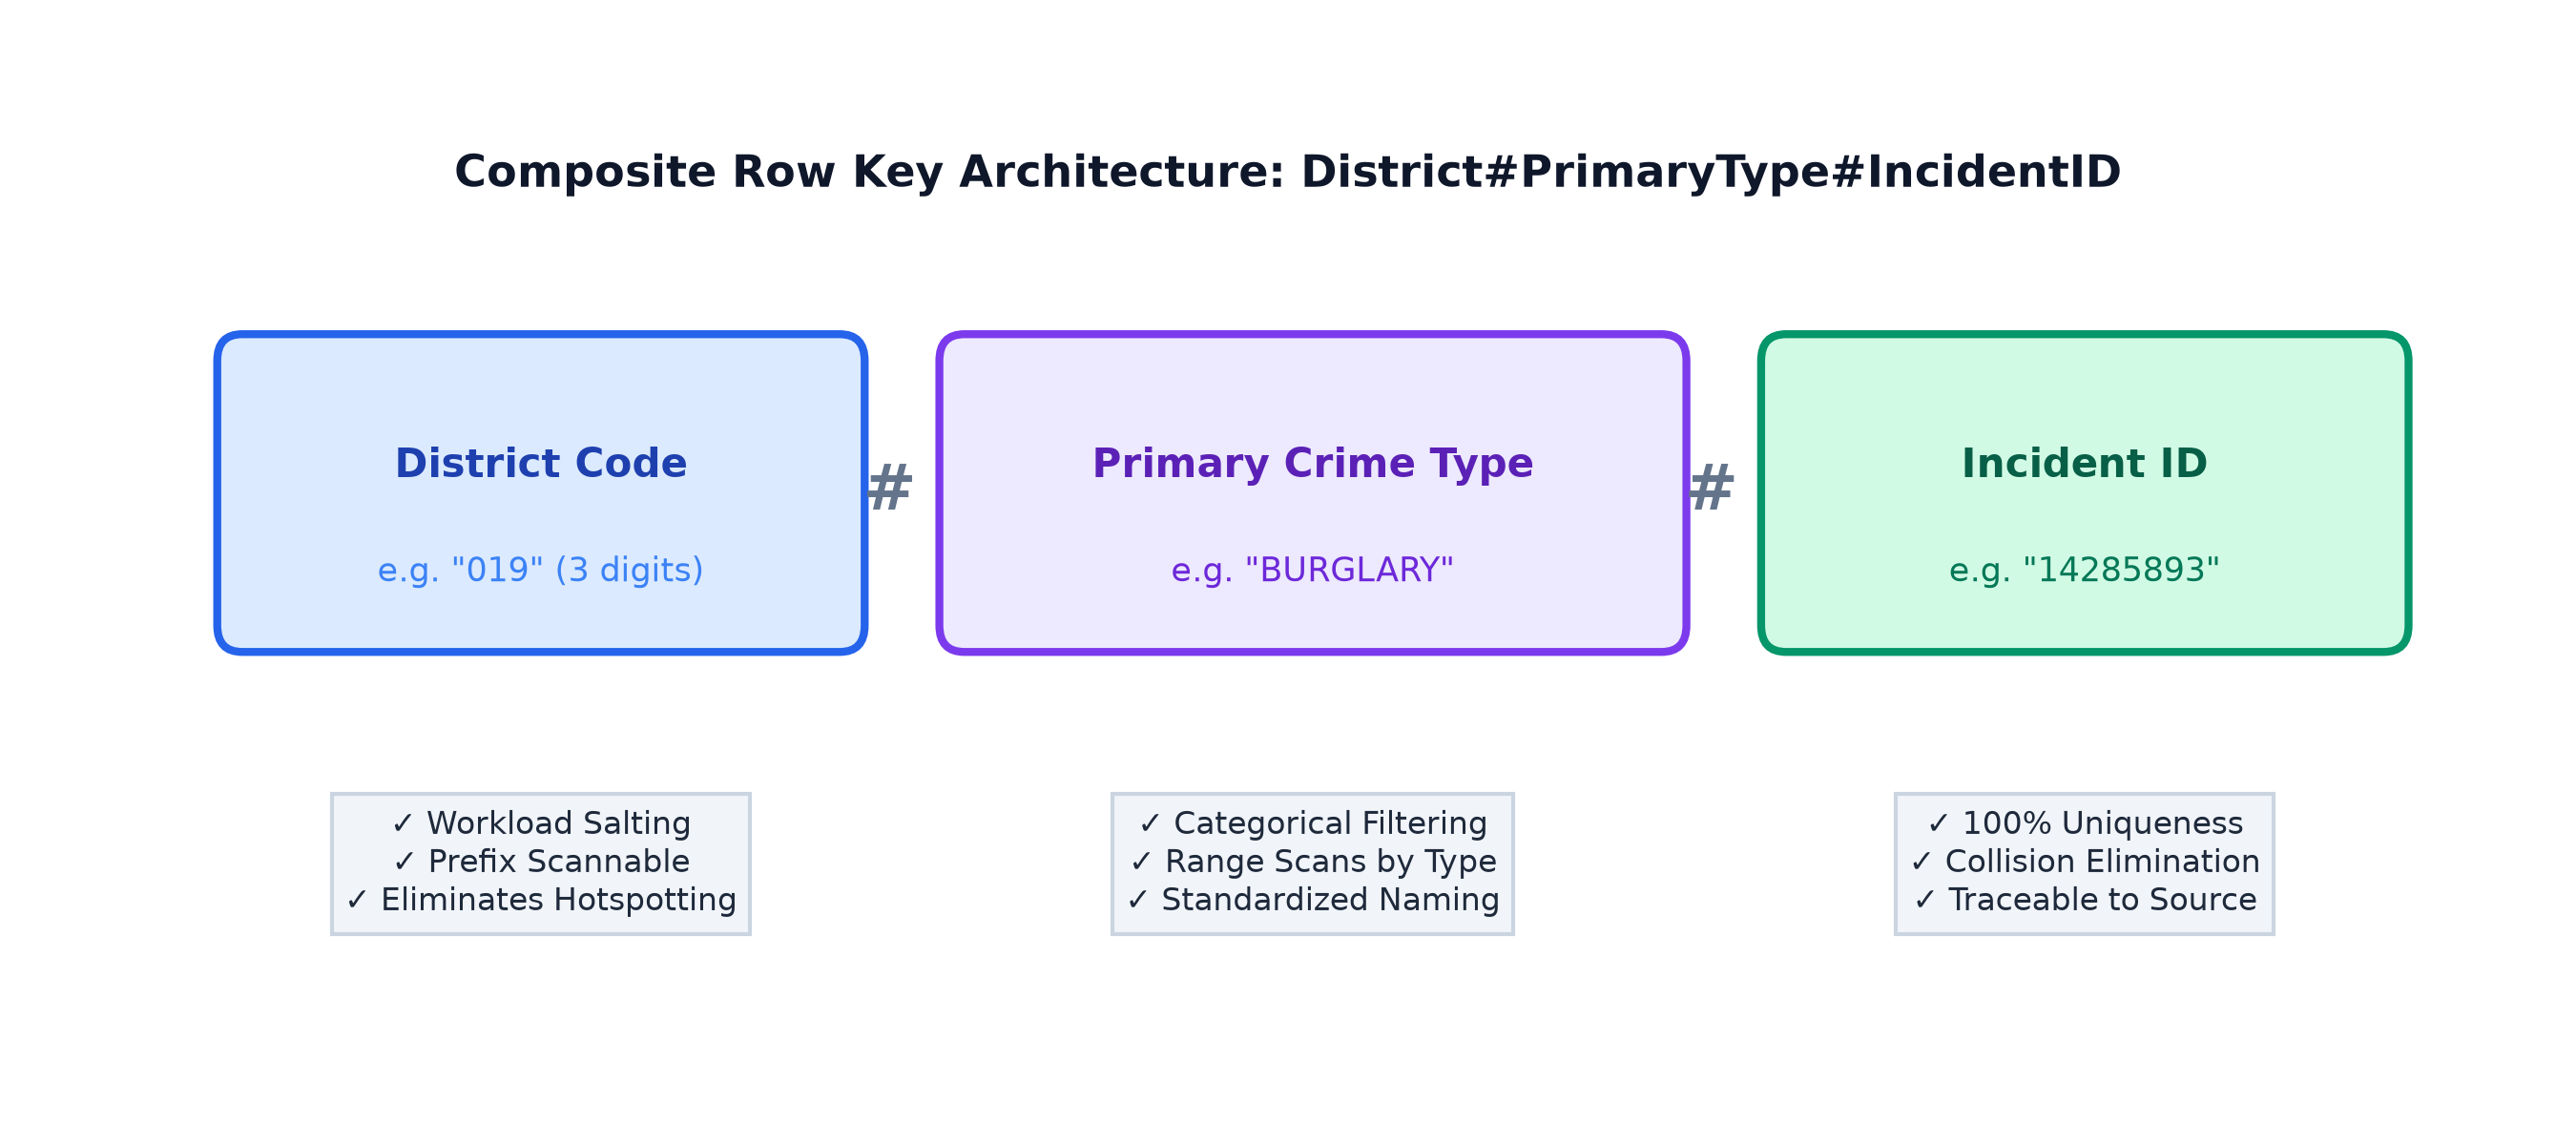
\includegraphics[height=1.8cm,keepaspectratio]{images/rowkey_design.png}
            \vspace{0.04cm}
            \par{\tiny\textit{Figure 2: Composite Row Key: \texttt{District\#CrimeType\#IncidentID}}}
            \vspace{0.04cm}
            \begin{itemize}\scriptsize
                \setlength{\itemsep}{2pt}
                \item \textbf{Anti-Hotspotting:} District prefix salts incoming writes evenly across RegionServers (eliminates timestamp hotspotting).
                \item \textbf{Prefix-Scannable:} Fast precinct-wide scans via \texttt{PrefixFilter('011\#')}.
                \item \textbf{Categorical Drill-Down:} Embedded crime type enables fast regex scans (e.g., \texttt{\^{}.*\#NARCOTICS\#.*}).
                \item \textbf{Uniqueness:} Incident ID suffix guarantees 100\% unique keys.
            \end{itemize}
        \end{column}
    \end{columns}
\end{frame}

% ==========================================================================
% SLIDE 5: Cluster Daemons Verification & 10,000 Record Batch Ingestion
% ==========================================================================
\begin{frame}{Step 3: Cluster Startup \& 10,000 Record Batch Ingestion}
    \begin{columns}[T]
        \begin{column}{0.48\textwidth}
            \textbf{\textcolor{NavyBlue}{1. HDFS \& HBase Daemons (\texttt{jps}):}}
            \vspace{0.04cm}
            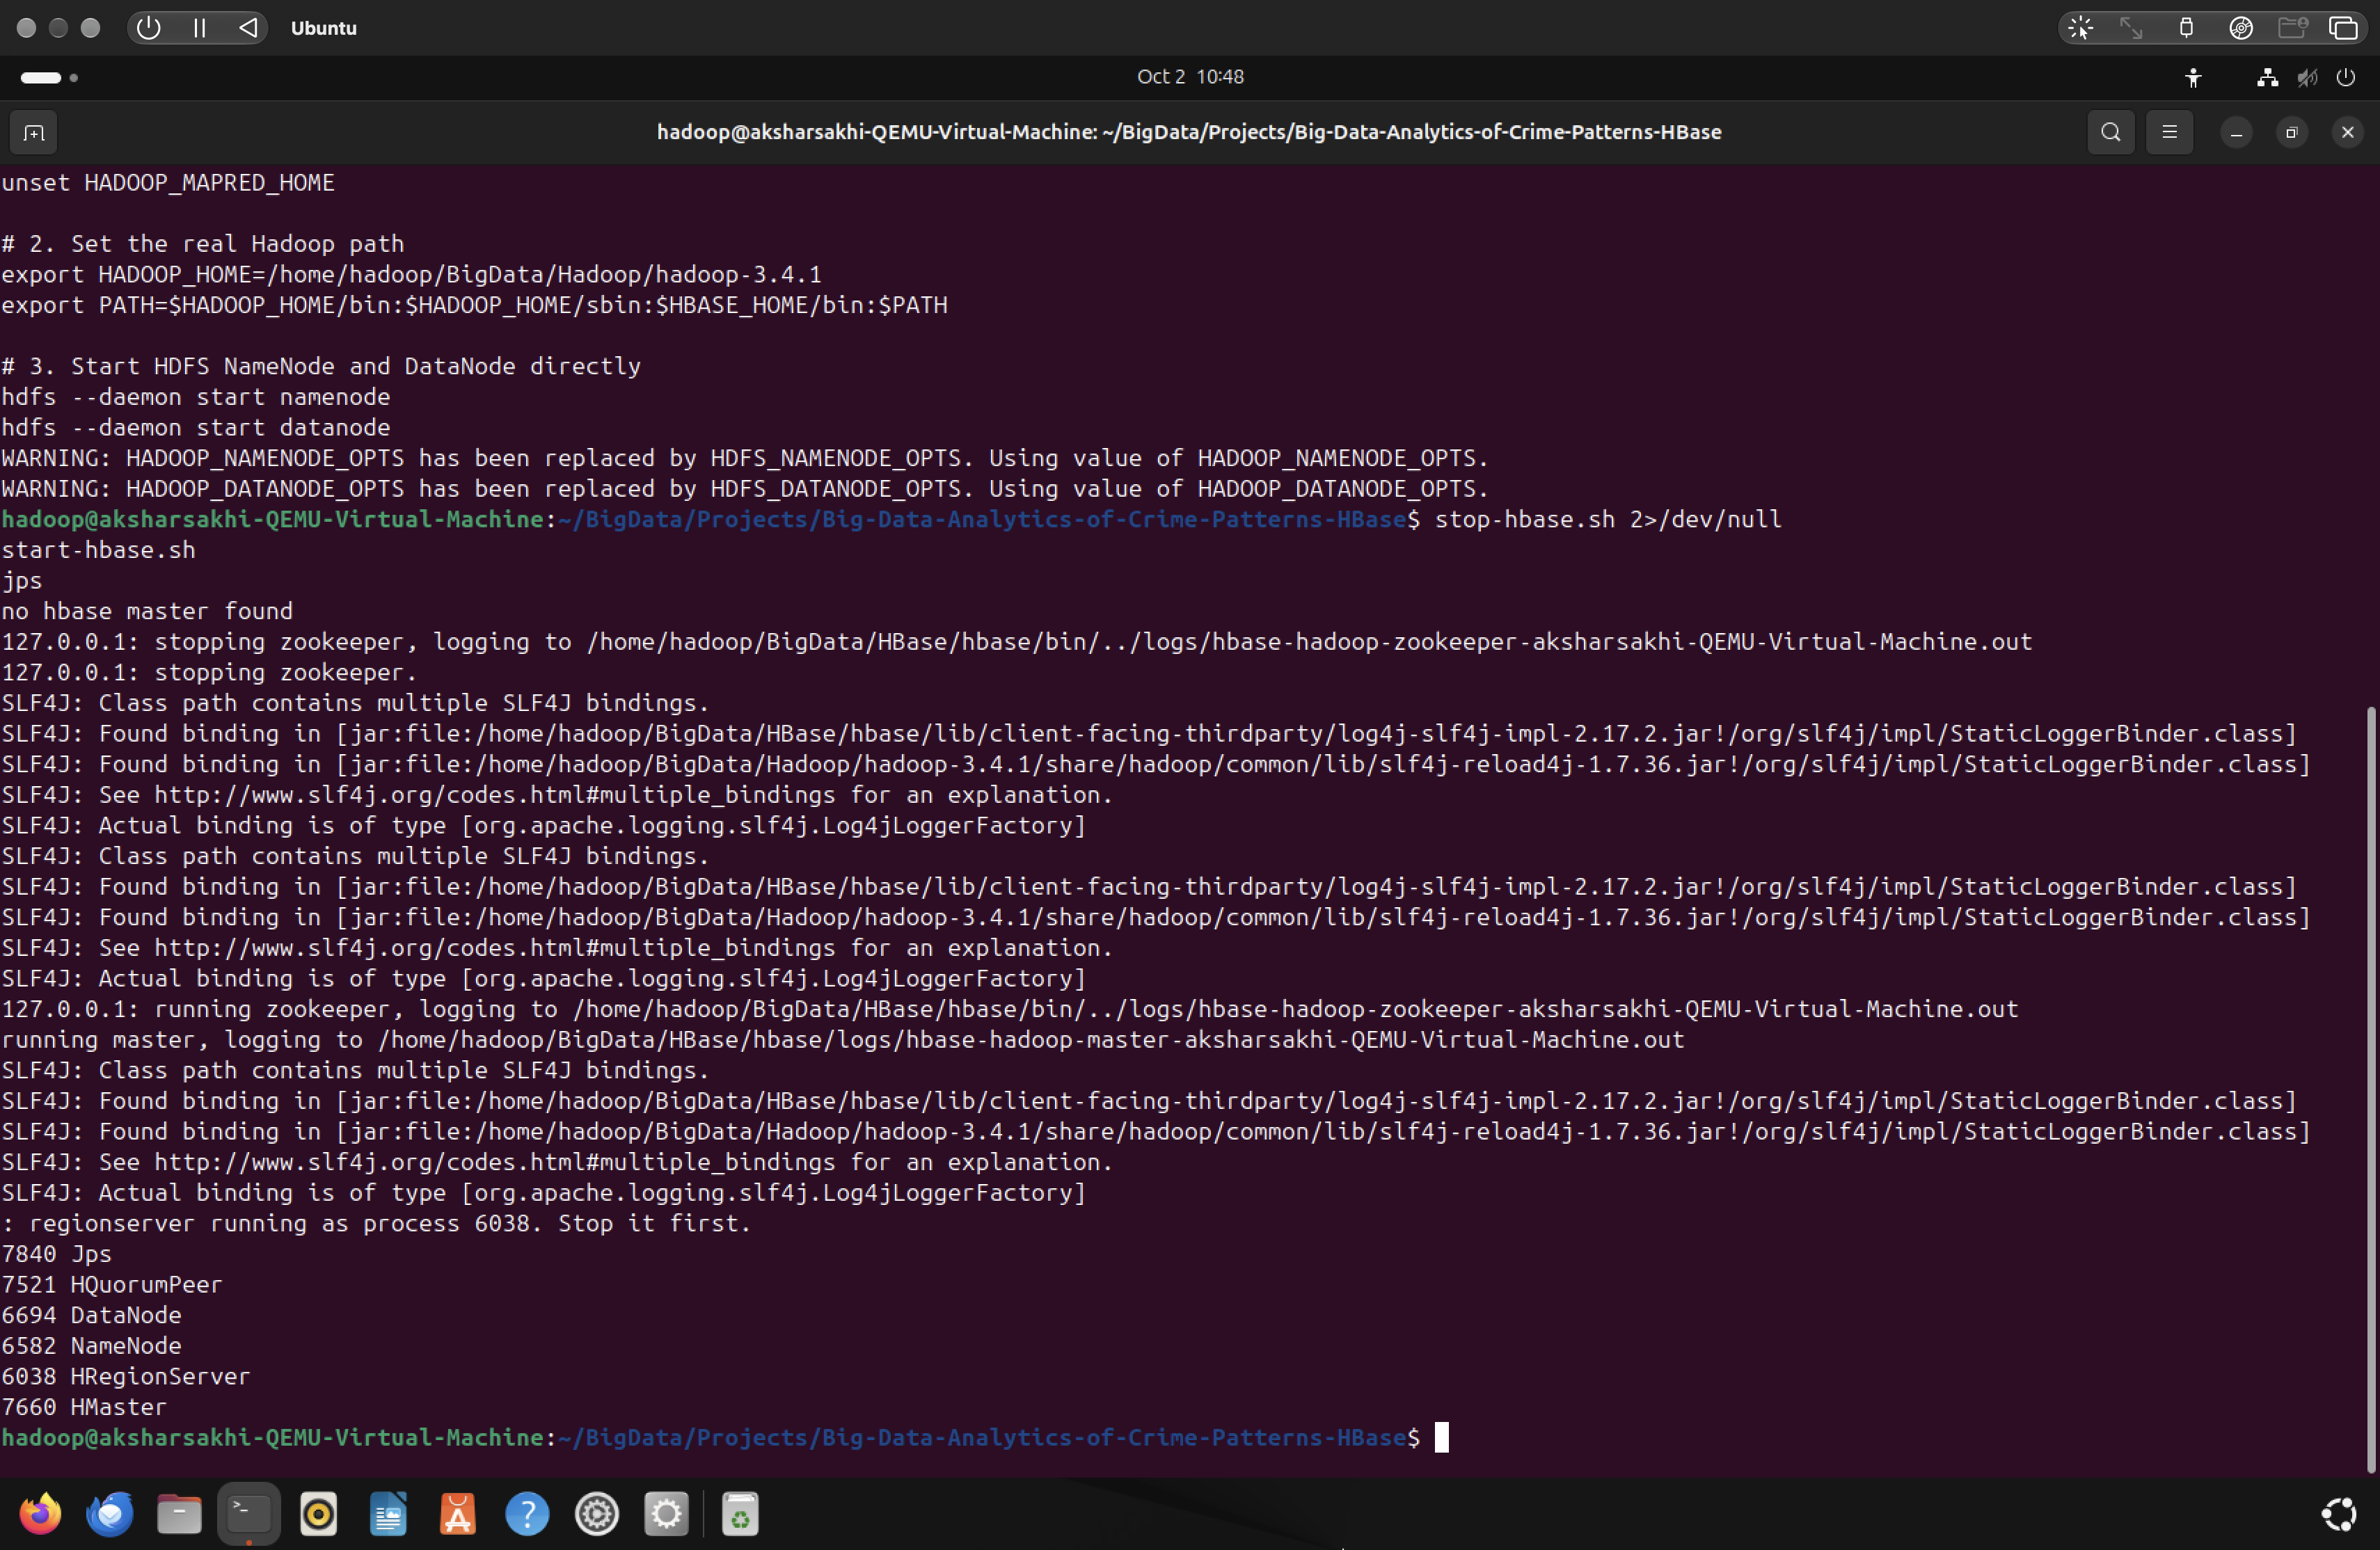
\includegraphics[width=\linewidth,height=4.4cm,keepaspectratio]{images/01_cluster_daemons_jps.png}
            \vspace{0.03cm}
            \begin{itemize}\tiny
                \setlength{\itemsep}{1pt}
                \item \textbf{HDFS Daemons:} \texttt{NameNode} (6582), \texttt{DataNode} (6694).
                \item \textbf{HBase Daemons:} \texttt{HQuorumPeer} (7521), \texttt{HMaster} (7660), \texttt{HRegionServer} (6038).
            \end{itemize}
        \end{column}
        \begin{column}{0.48\textwidth}
            \textbf{\textcolor{NavyBlue}{2. Batch Ingestion (\texttt{populate\_hbase.sh}):}}
            \vspace{0.04cm}
            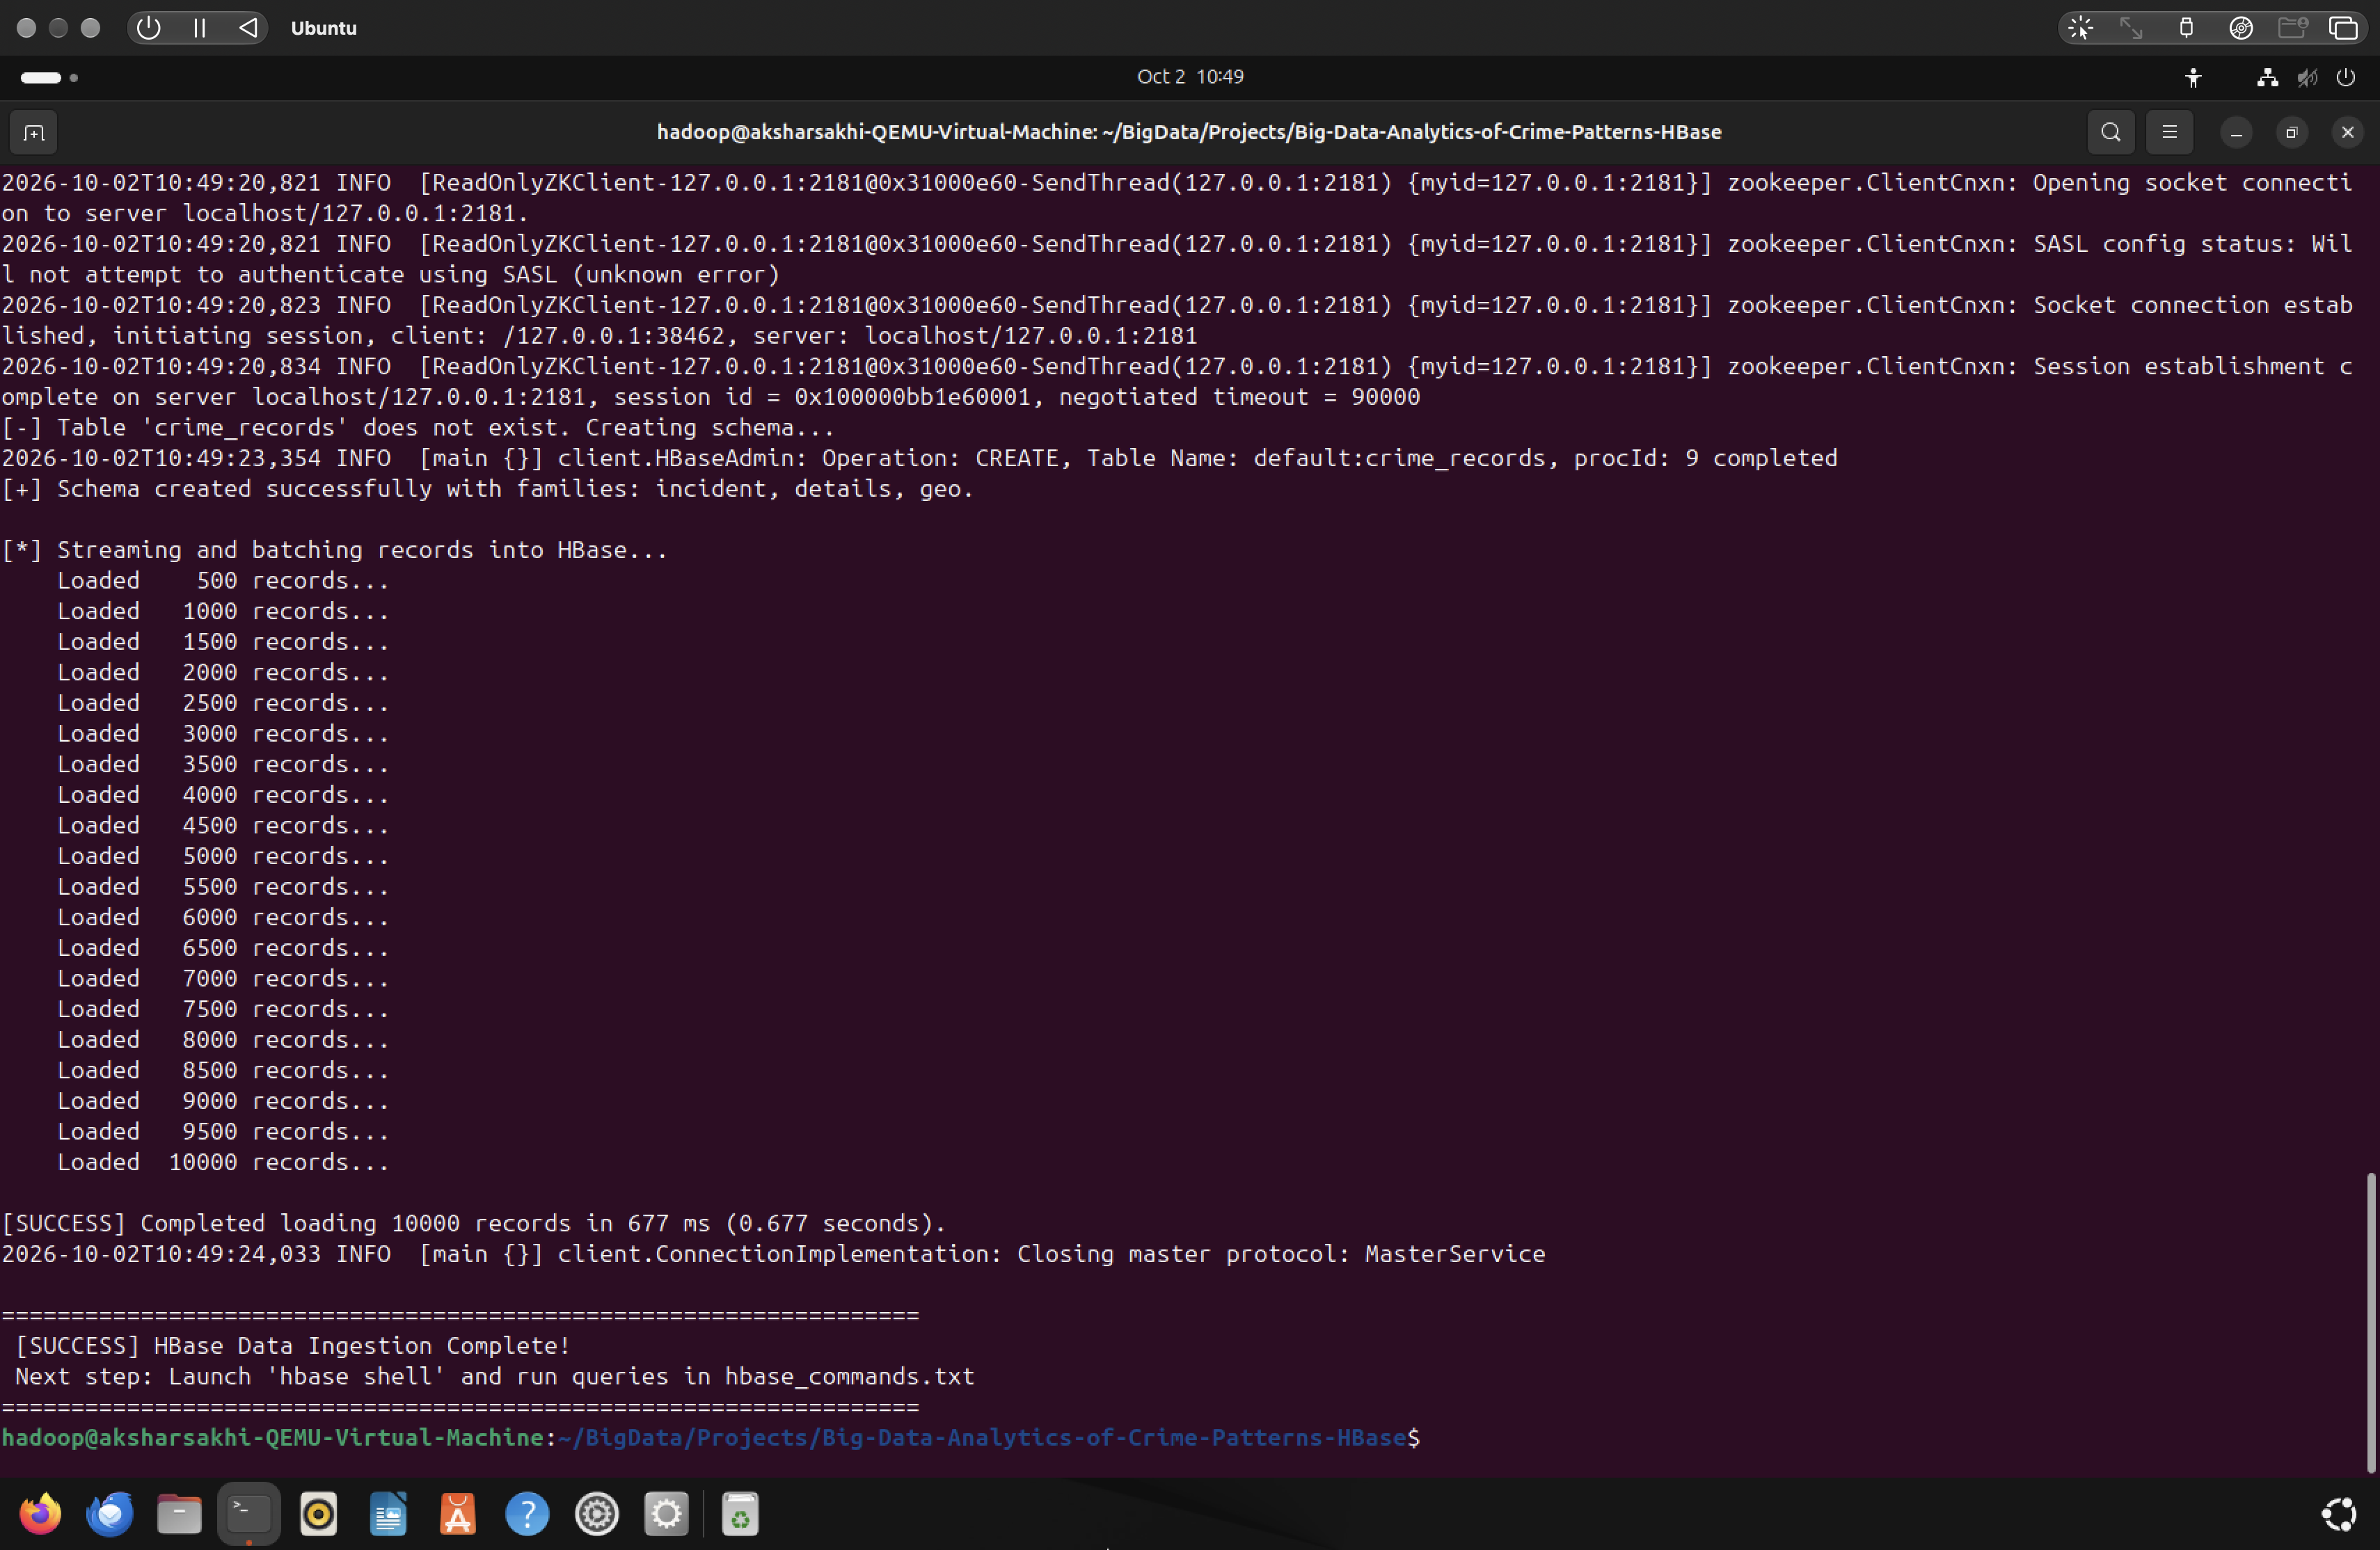
\includegraphics[width=\linewidth,height=4.4cm,keepaspectratio]{images/02_data_ingestion_10k_records.png}
            \vspace{0.03cm}
            \begin{itemize}\tiny
                \setlength{\itemsep}{1pt}
                \item \textbf{Batch Loader:} 500 records per RPC batch via \texttt{HBaseDataLoader}.
                \item \textbf{Throughput:} Loaded \textbf{10,000 authentic records in 677 ms} (0.677 seconds) directly into table \texttt{crime\_records}.
            \end{itemize}
        \end{column}
    \end{columns}
\end{frame}

% ==========================================================================
% SLIDE 6: HBase Command 1: Point Lookup Retrieval (GET)
% ==========================================================================
\begin{frame}[fragile]{Step 4: HBase Shell Command 1 -- Point Lookup (\texttt{GET})}
    \noindent\colorbox{LightGray}{\parbox{\dimexpr\linewidth-2\fboxsep\relax}{%
        \scriptsize\textbf{Executed Command:} \texttt{get 'crime\_records', '019\#BURGLARY\#14285893'}%
    }}
    \vspace{0.08cm}
    \begin{columns}[T]
        \begin{column}{0.48\textwidth}
            \textbf{\textcolor{NavyBlue}{Schema Verification (\texttt{describe}):}}
            \vspace{0.04cm}
            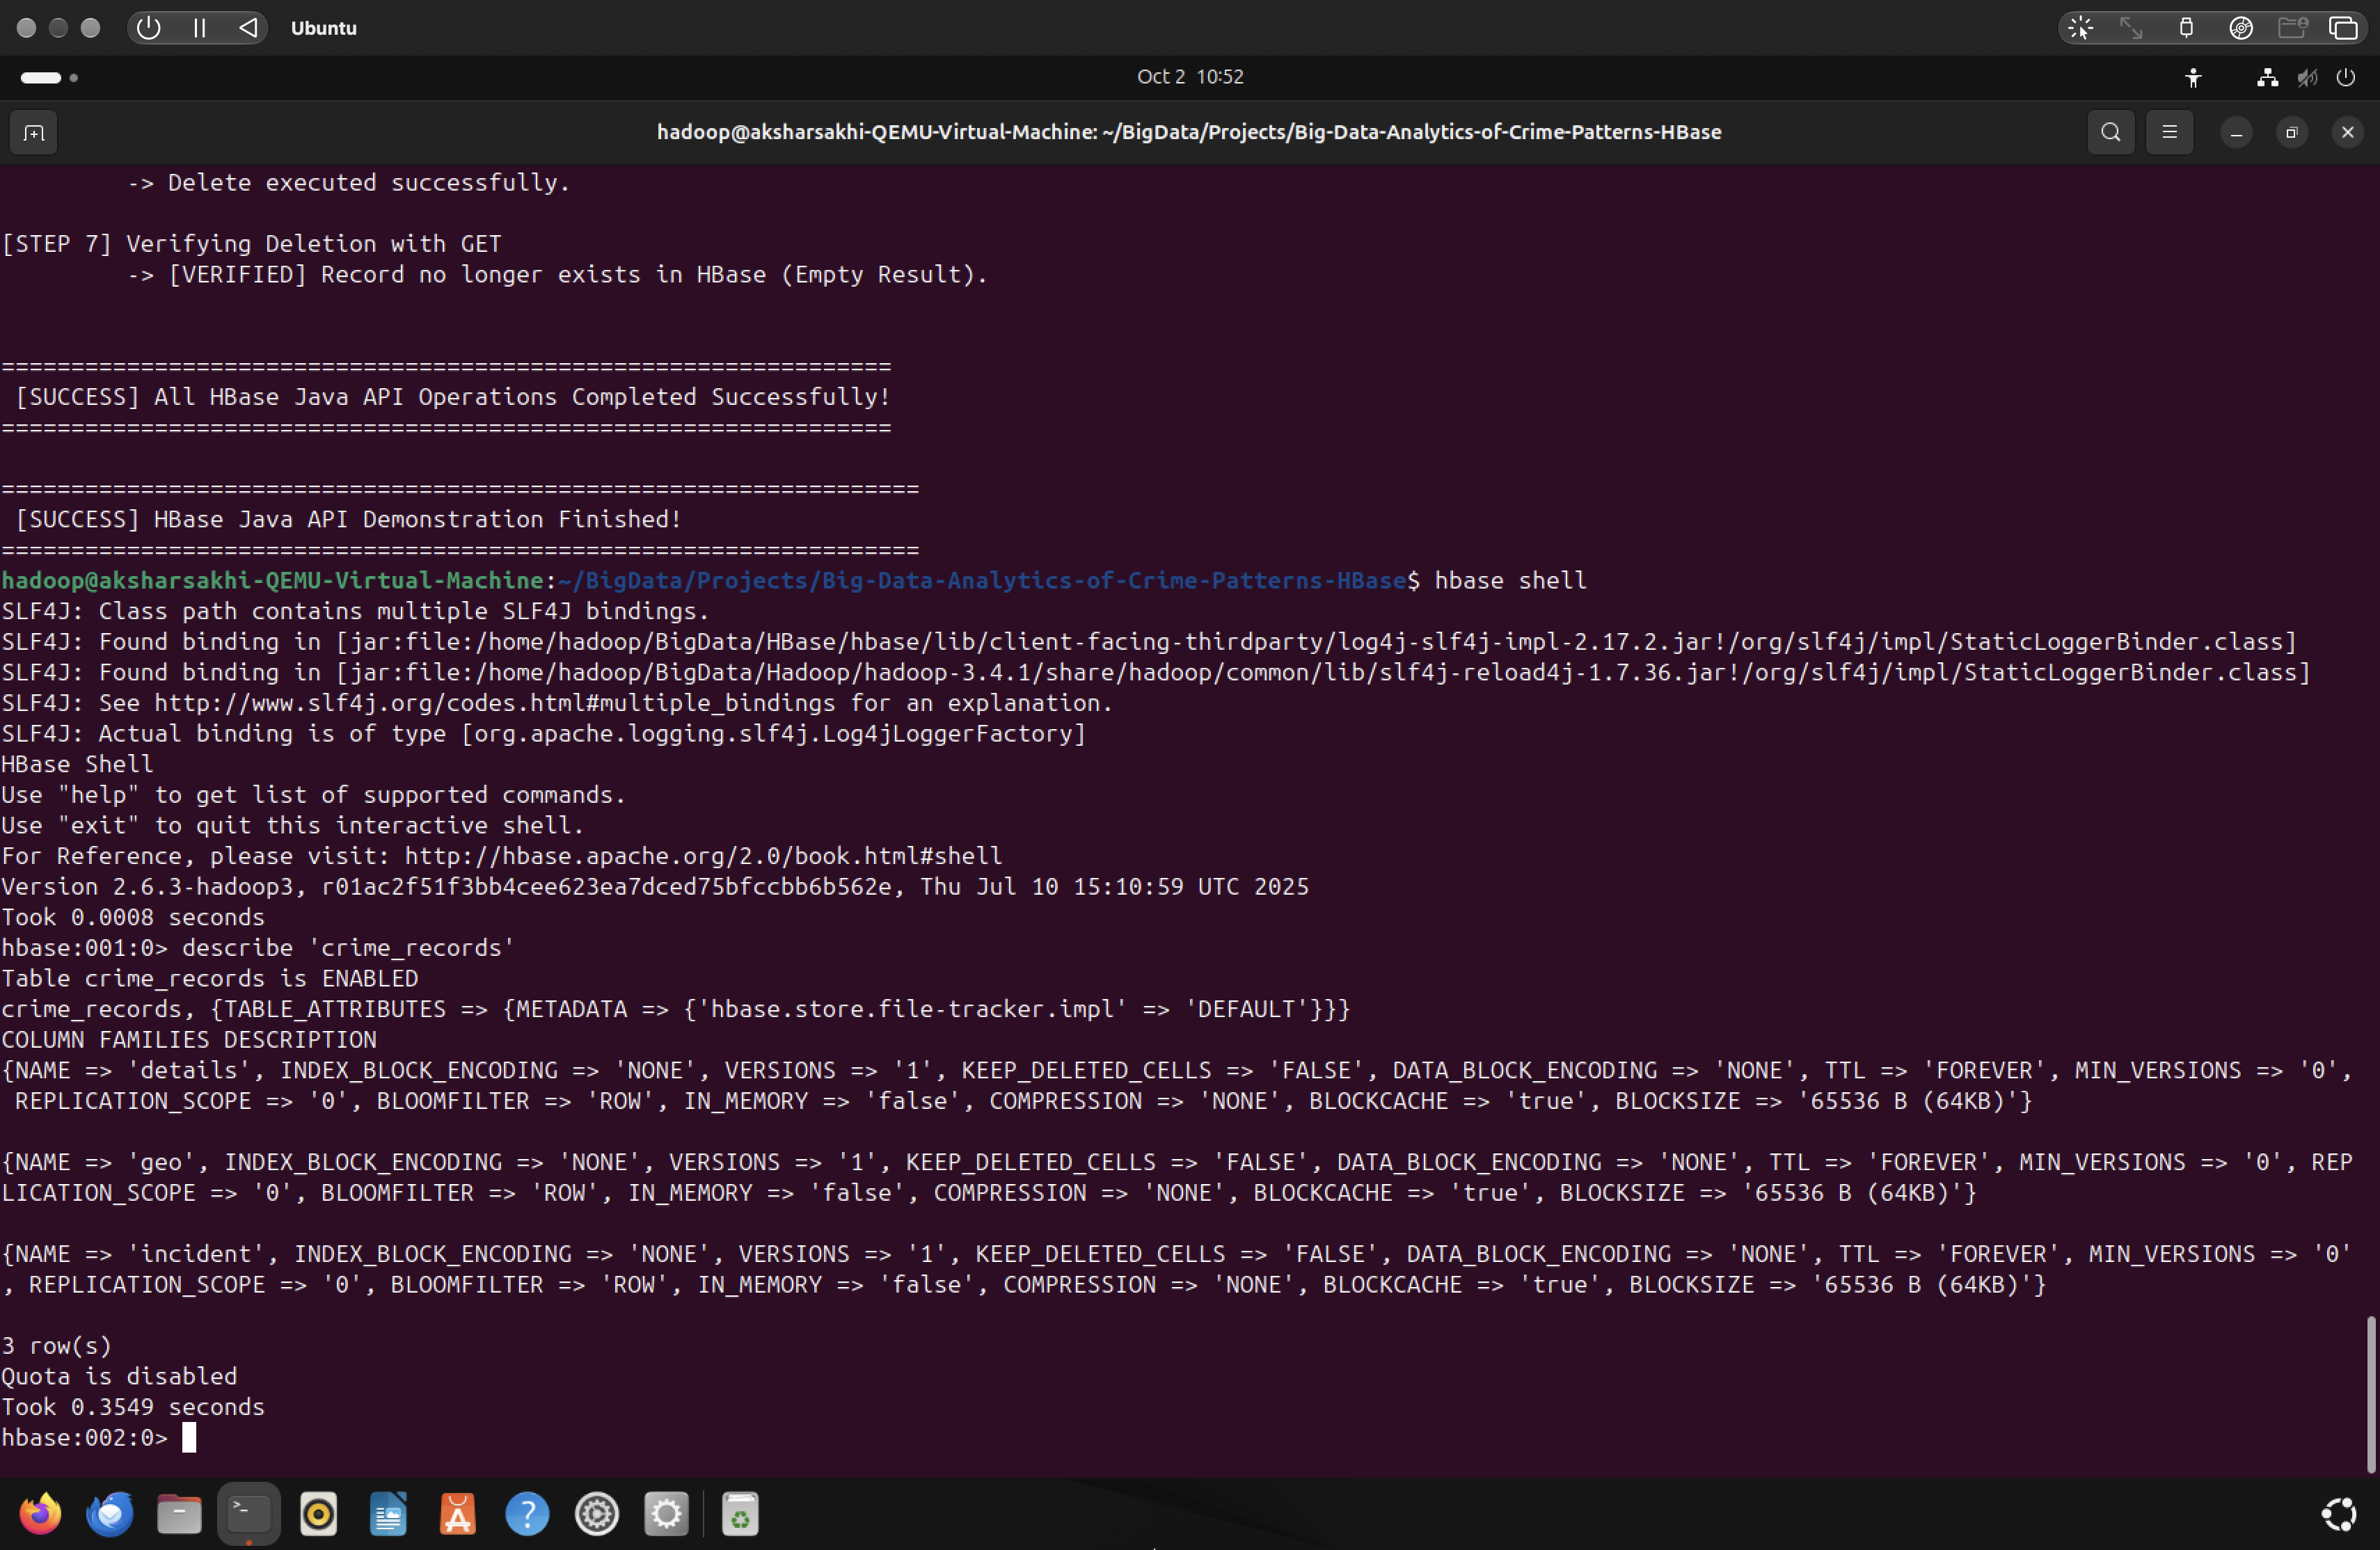
\includegraphics[width=\linewidth,height=4.1cm,keepaspectratio]{images/04_hbase_shell_describe_schema.png}
            \vspace{0.03cm}
            \begin{itemize}\tiny
                \setlength{\itemsep}{1.5pt}
                \item \textbf{Schema Check:} Confirms table is active with 3 column families (\texttt{incident}, \texttt{details}, \texttt{geo}) and BlockCache active.
                \item \textbf{Storage Indexing:} Row-key architecture enables direct memory lookup without scanning the table.
            \end{itemize}
        \end{column}
        \begin{column}{0.48\textwidth}
            \textbf{\textcolor{NavyBlue}{Point Lookup Result (\texttt{GET}):}}
            \vspace{0.04cm}
            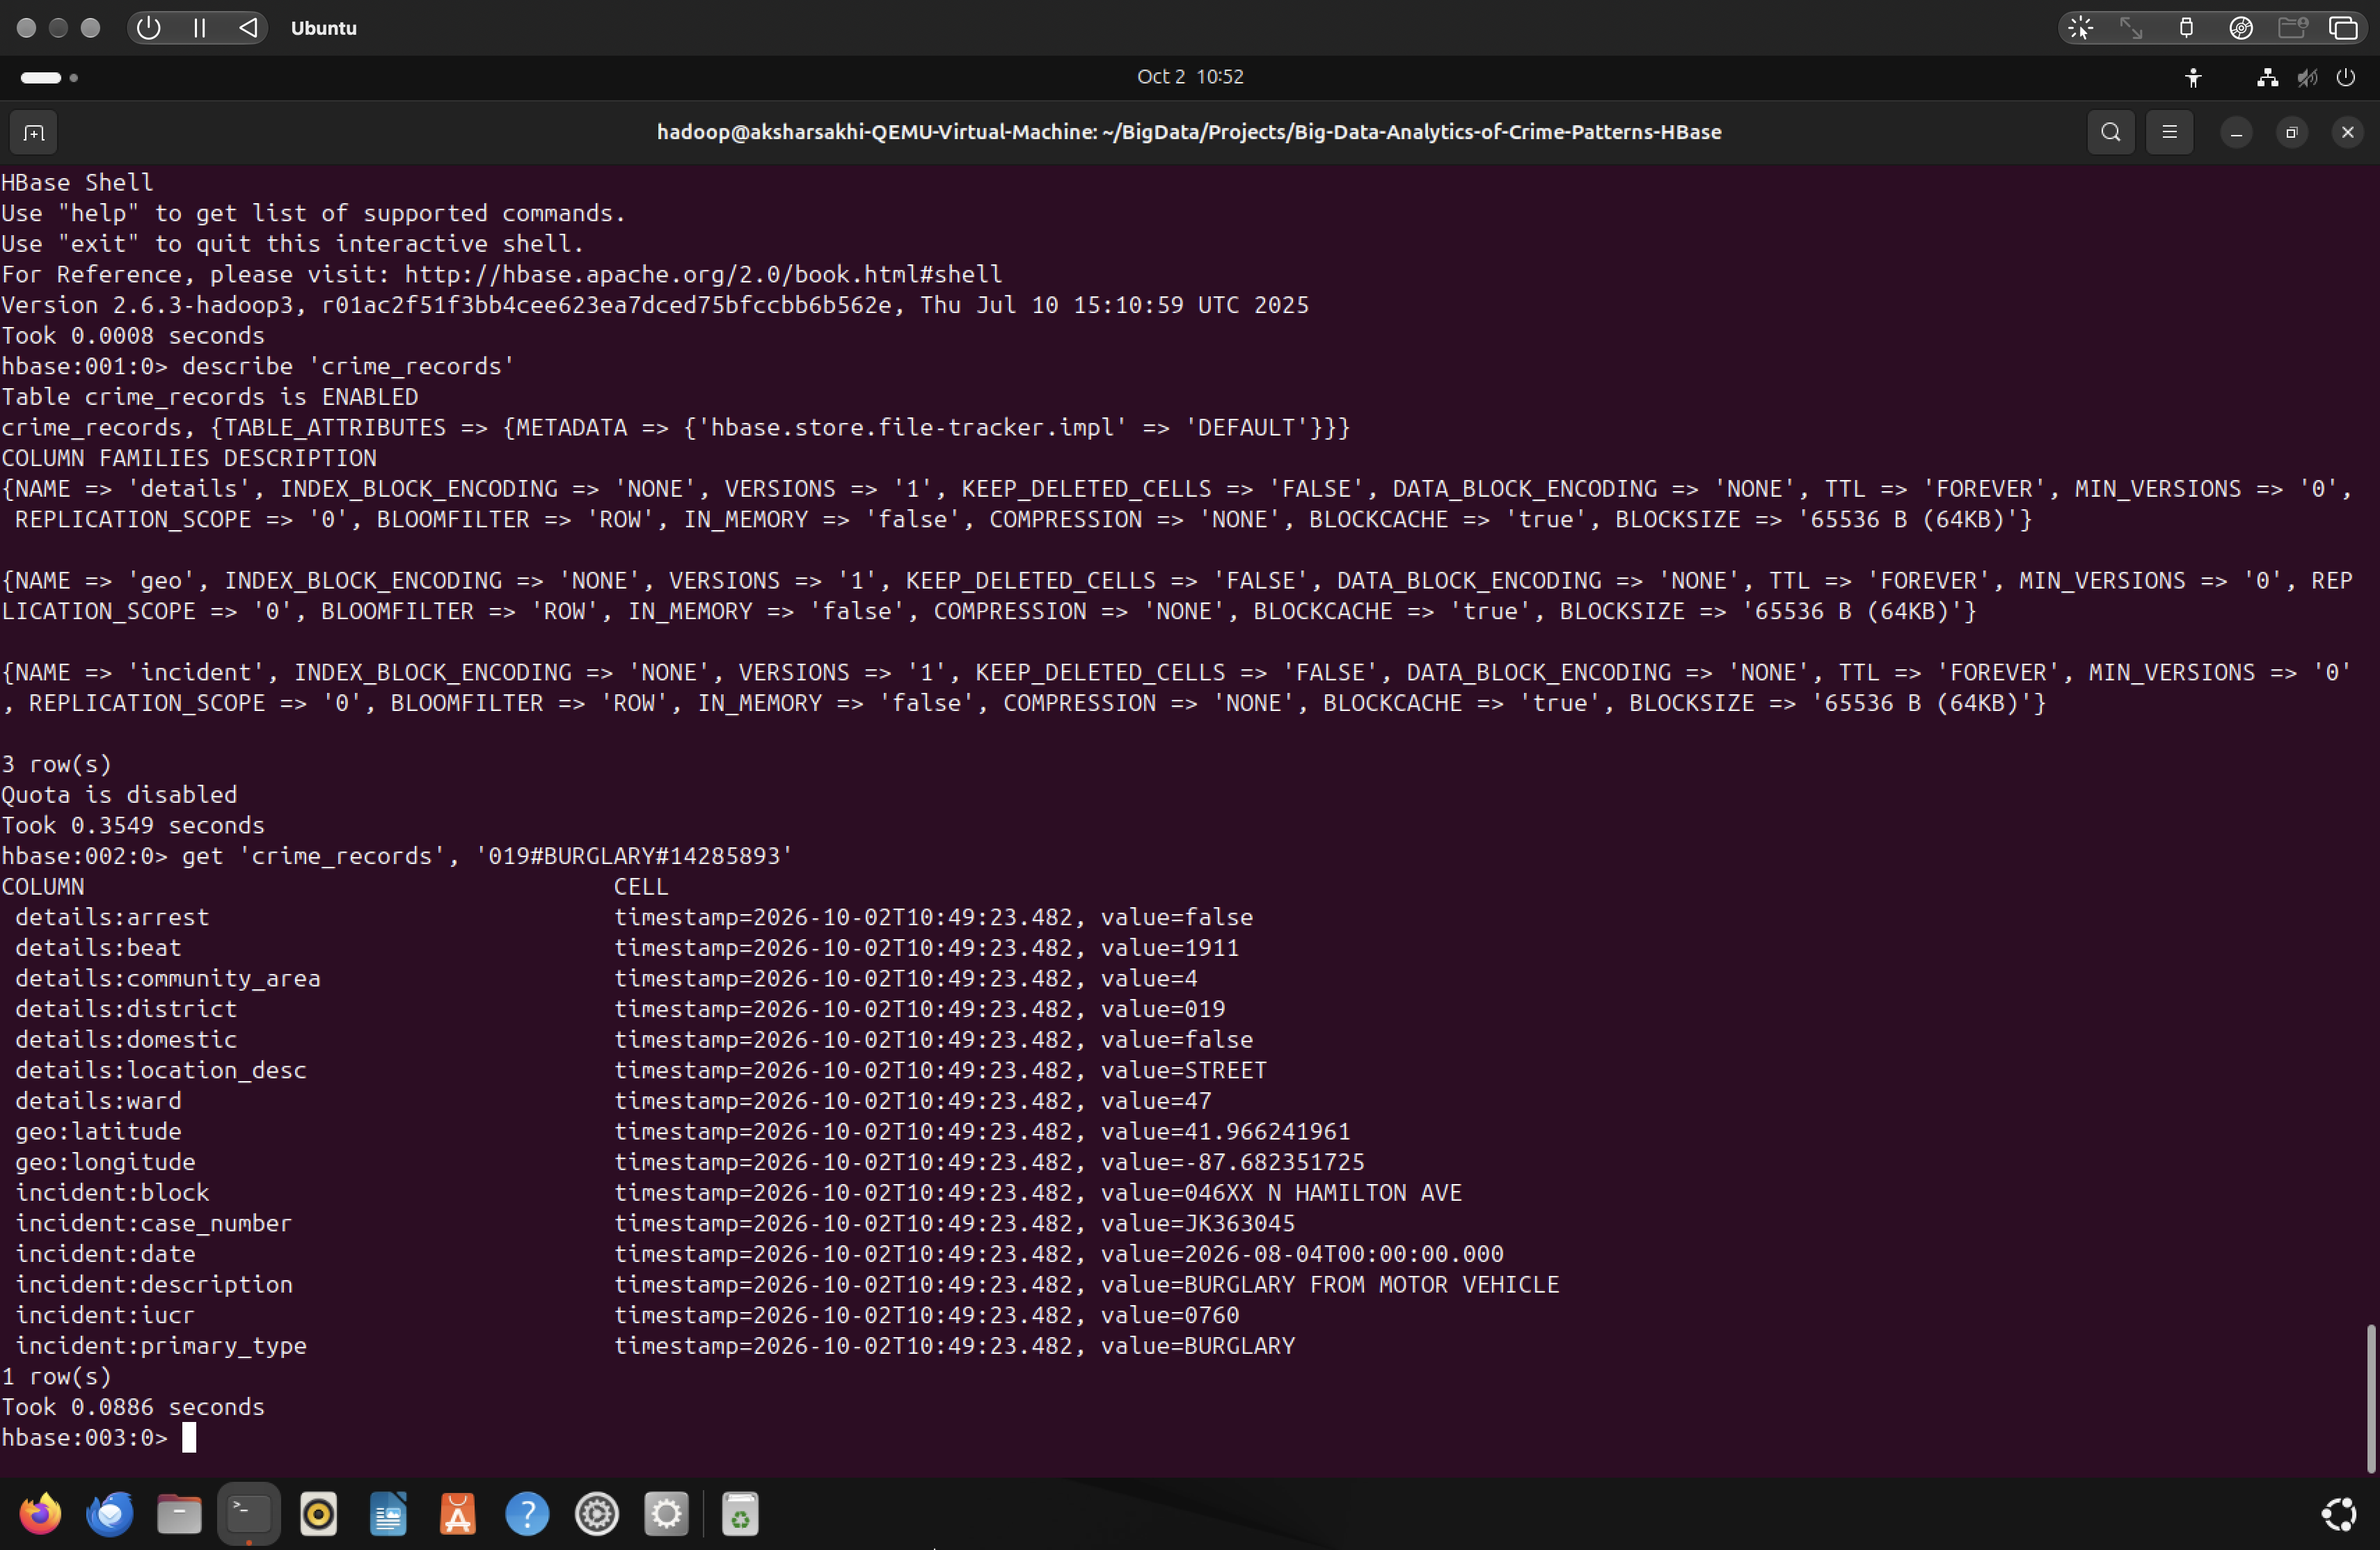
\includegraphics[width=\linewidth,height=4.1cm,keepaspectratio]{images/05_hbase_shell_get_record.png}
            \vspace{0.03cm}
            \begin{itemize}\tiny
                \setlength{\itemsep}{1.5pt}
                \item \textbf{Targeted Lookup:} Random access by composite key (\texttt{District\#Type\#ID}) fetching all 14 attributes in \textbf{0.0886 seconds}.
                \item \textbf{Field Output:} Instantly retrieves case number, arrest status, beat, and GPS coordinates for field units.
            \end{itemize}
        \end{column}
    \end{columns}
\end{frame}

% ==========================================================================
% SLIDE 7: HBase Command 2: SingleColumnValueFilter (Arrest Tracking)
% ==========================================================================
\begin{frame}[fragile]{Step 4: HBase Shell Command 2 -- \texttt{SingleColumnValueFilter}}
    \noindent\colorbox{LightGray}{\parbox{\dimexpr\linewidth-2\fboxsep\relax}{%
        \tiny\textbf{Executed Command:} \texttt{scan 'crime\_records', \{FILTER => "SingleColumnValueFilter('details', 'arrest', =, 'binary:true')", LIMIT => 3\}}%
    }}
    \vspace{0.04cm}
    \begin{columns}[T]
        \begin{column}{0.49\textwidth}
            \textbf{\textcolor{NavyBlue}{\scriptsize (a) Query Invocation \& Initial Matching Rows:}}
            \vspace{0.02cm}
            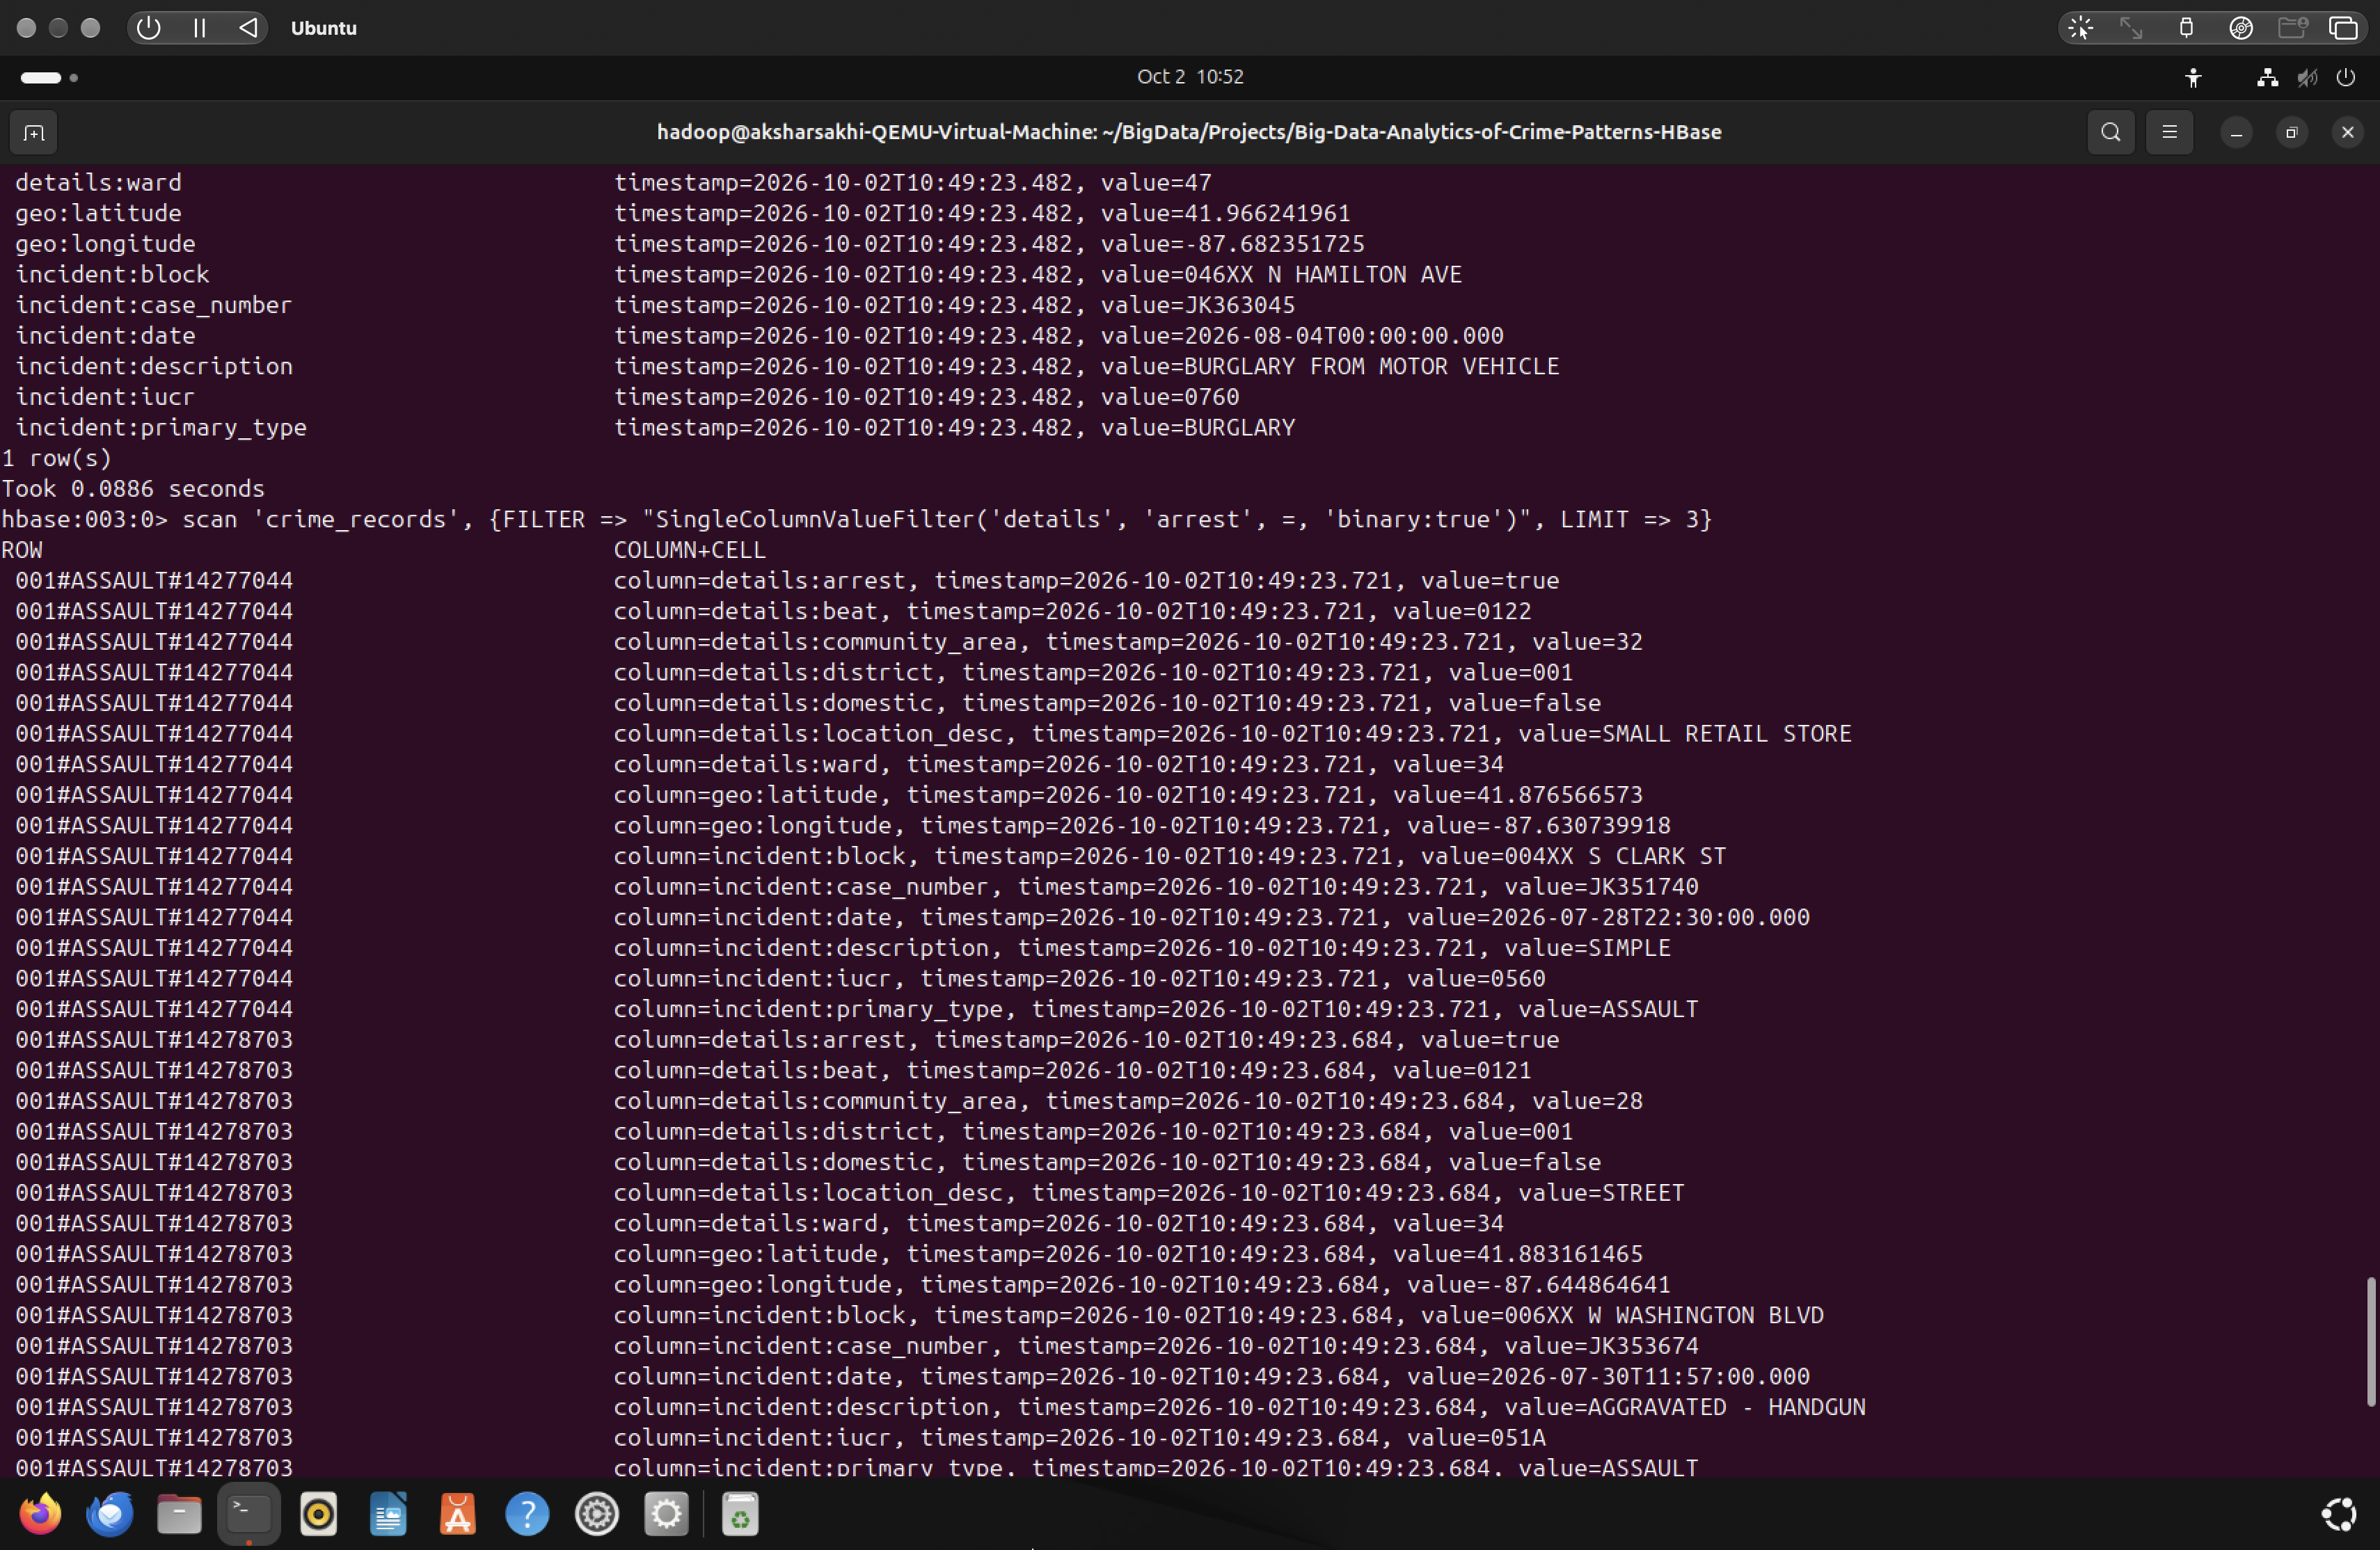
\includegraphics[width=\linewidth,height=3.35cm,keepaspectratio]{images/06_hbase_filter_arrest_scan_pt1.png}
        \end{column}
        \begin{column}{0.49\textwidth}
            \textbf{\textcolor{NavyBlue}{\scriptsize (b) Result Continuation \& Timing (0.0711s):}}
            \vspace{0.02cm}
            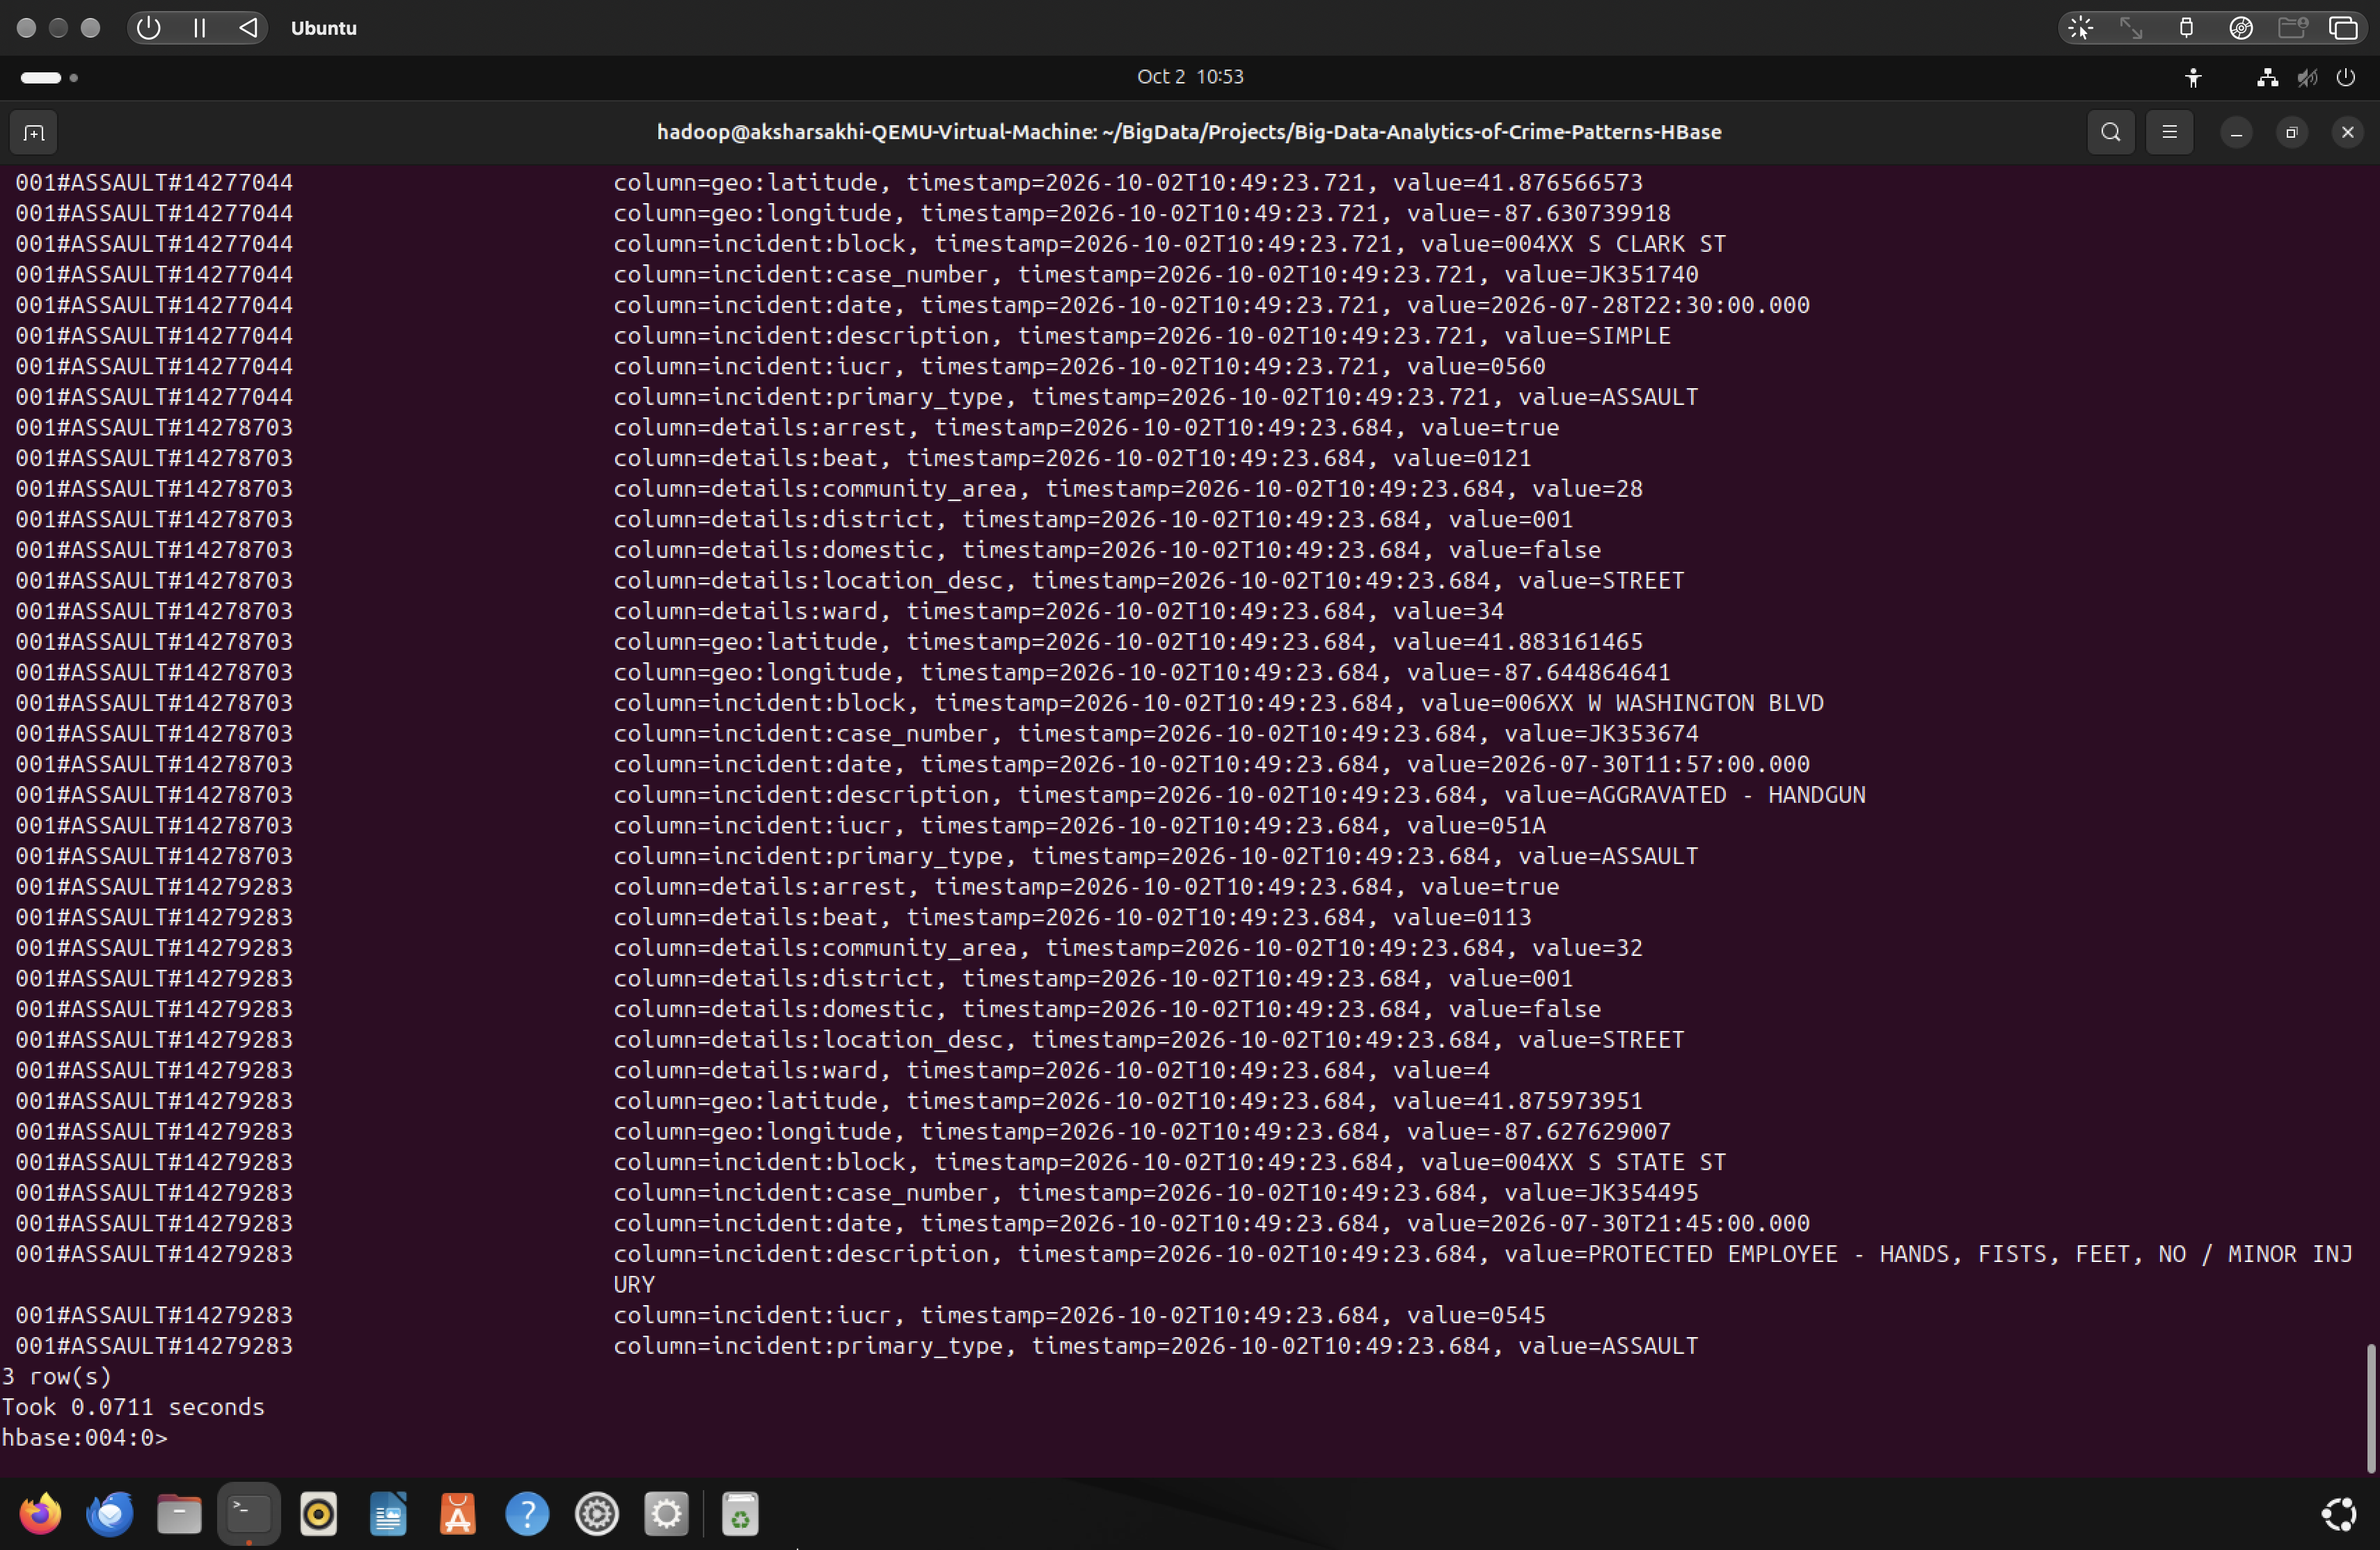
\includegraphics[width=\linewidth,height=3.35cm,keepaspectratio]{images/07_hbase_filter_arrest_scan_pt2.png}
        \end{column}
    \end{columns}
    \vspace{0.03cm}
    \begin{itemize}\scriptsize
        \setlength{\itemsep}{1pt}
        \item \textbf{Server-Side Filtering:} Evaluates \texttt{details:arrest = 'true'} directly on RegionServers across 10,000 rows.
        \item \textbf{Zero Network Overhead:} Returns matching incidents in \textbf{0.0711 seconds}, discarding unapprehended rows at source.
        \item \textbf{Operational Value:} Enables law enforcement to instantly track solved cases and apprehend rates per district.
    \end{itemize}
\end{frame}

% ==========================================================================
% SLIDE 8: HBase Command 3: PrefixFilter (District Jurisdiction Scan)
% ==========================================================================
\begin{frame}[fragile]{Step 4: HBase Shell Command 3 -- \texttt{PrefixFilter} (District Scan)}
    \noindent\colorbox{LightGray}{\parbox{\dimexpr\linewidth-2\fboxsep\relax}{%
        \scriptsize\textbf{Executed Command:} \texttt{scan 'crime\_records', \{FILTER => "PrefixFilter('011\#')", LIMIT => 3\}}%
    }}
    \vspace{0.04cm}
    \begin{columns}[T]
        \begin{column}{0.49\textwidth}
            \textbf{\textcolor{NavyBlue}{\scriptsize (a) Query Invocation \& Initial District Records:}}
            \vspace{0.02cm}
            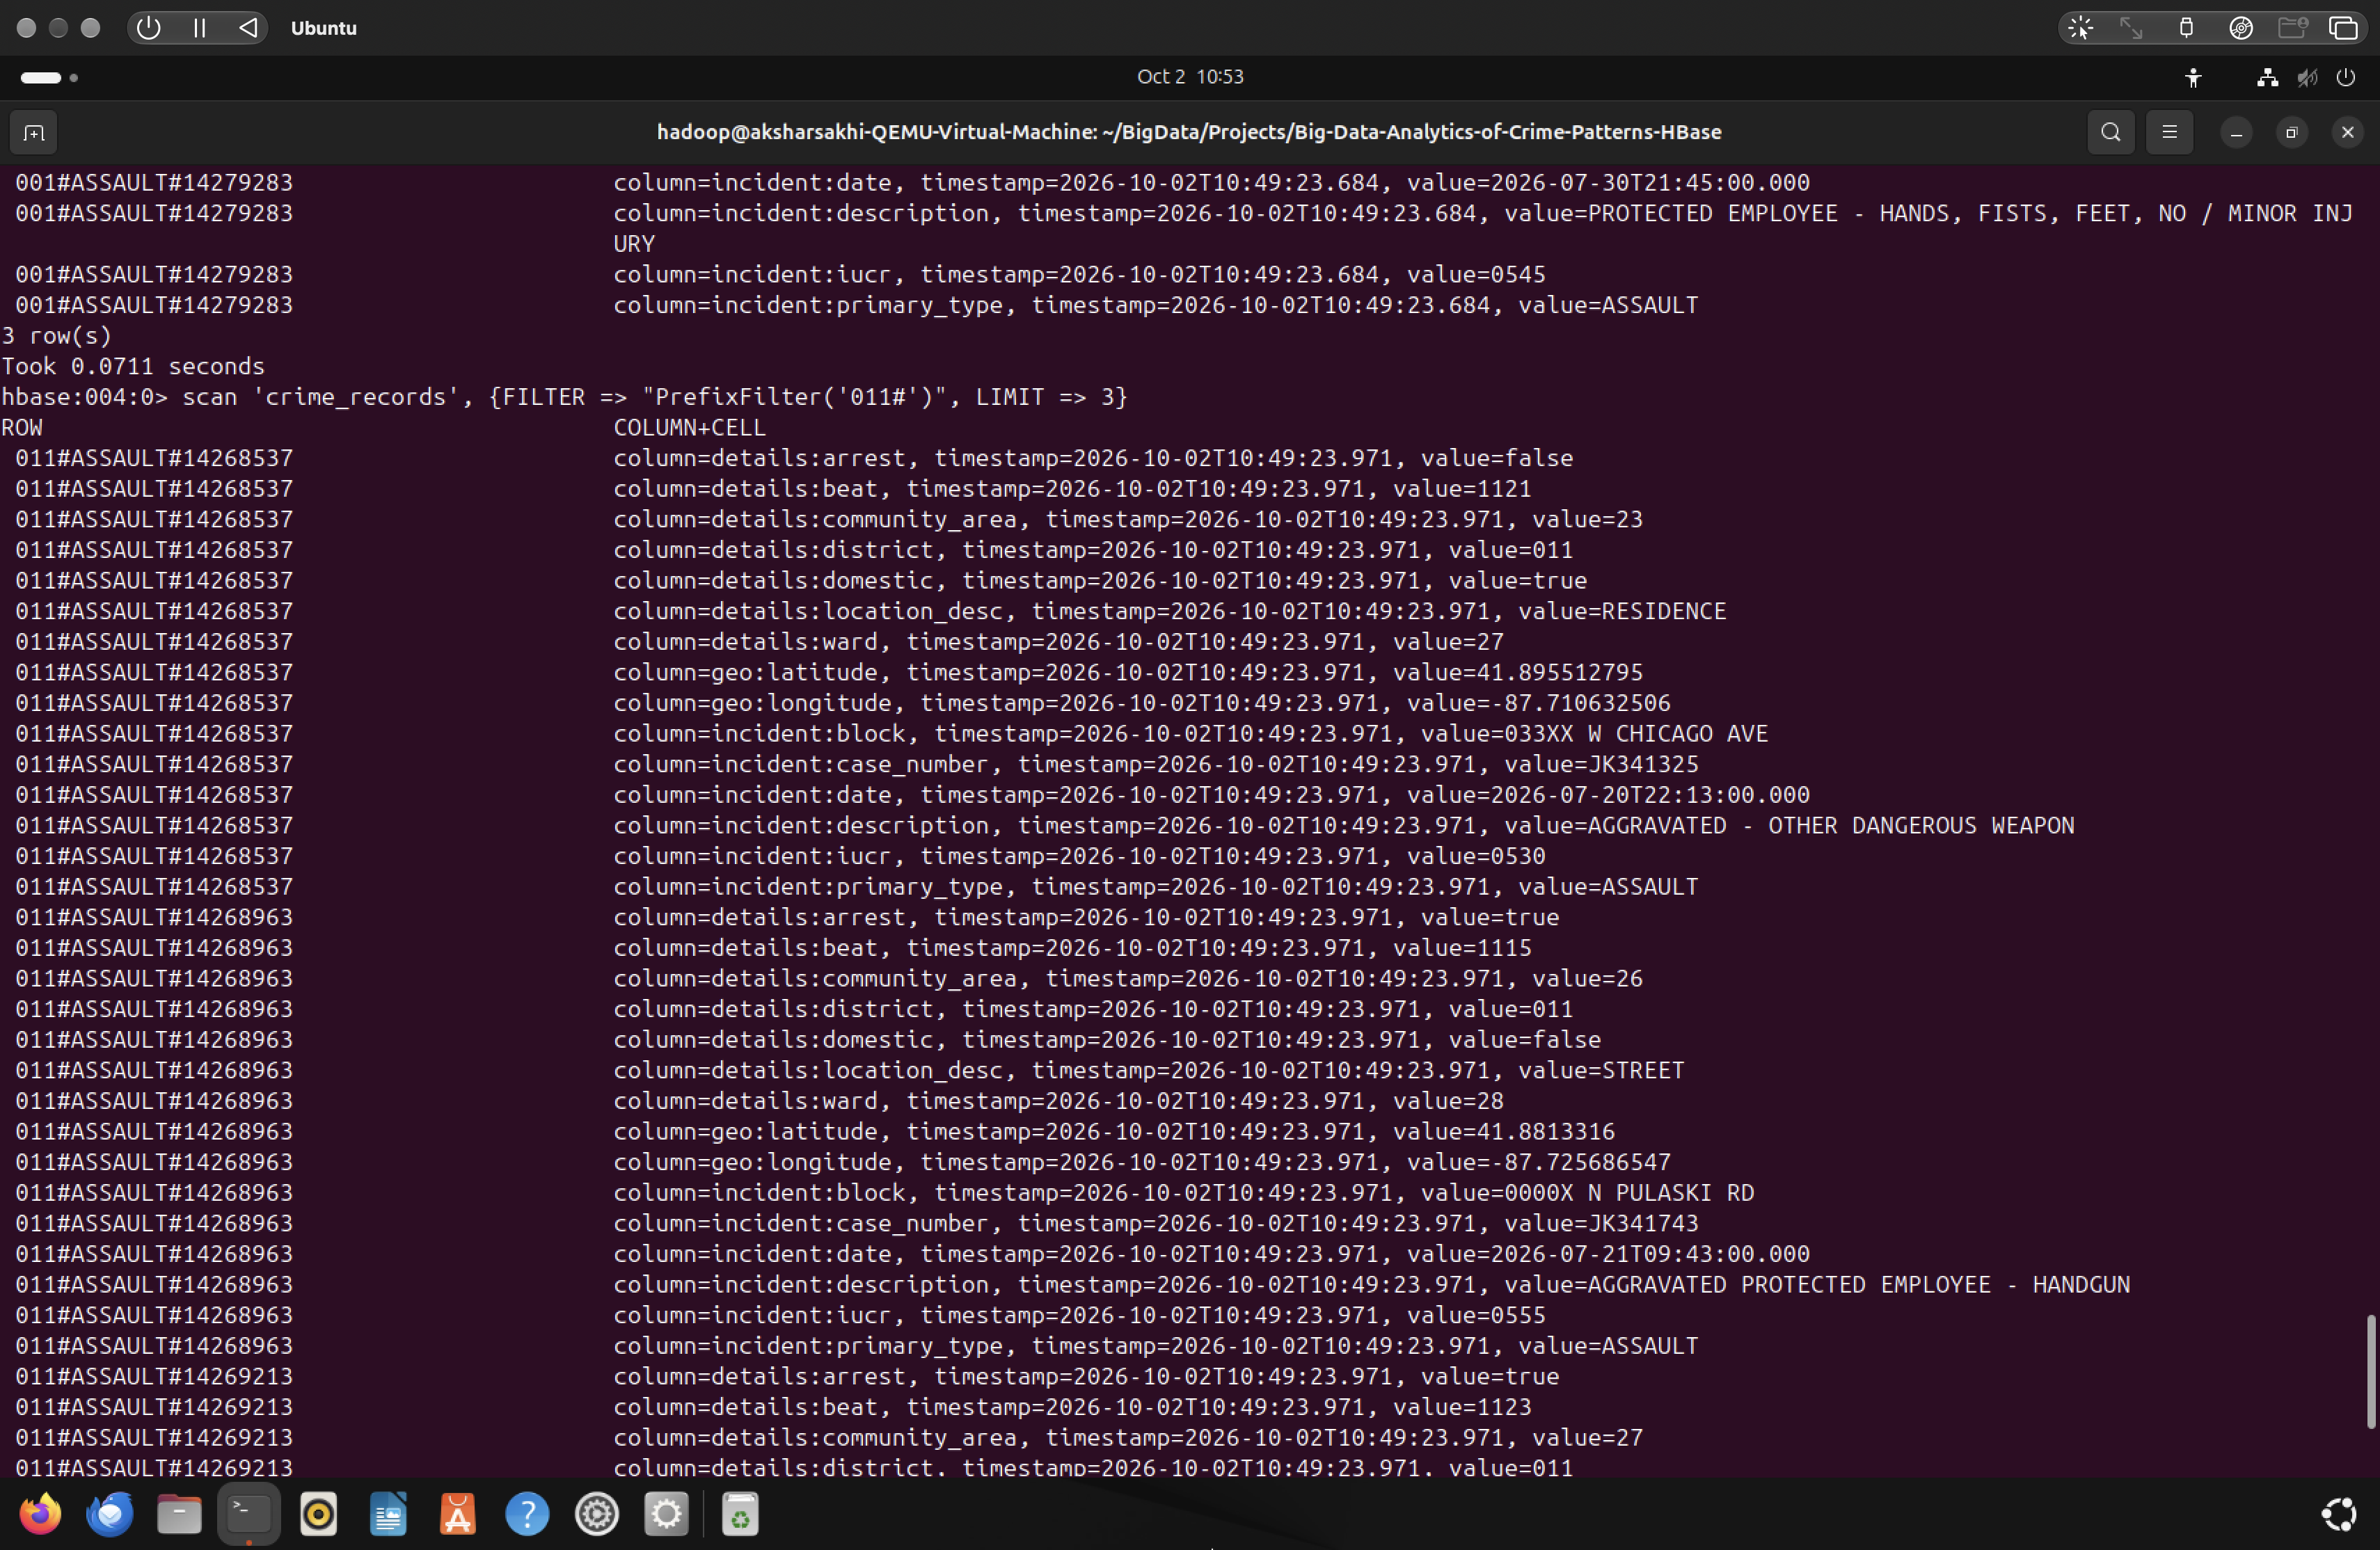
\includegraphics[width=\linewidth,height=3.35cm,keepaspectratio]{images/08_hbase_filter_prefix_011_pt1.png}
        \end{column}
        \begin{column}{0.49\textwidth}
            \textbf{\textcolor{NavyBlue}{\scriptsize (b) Result Continuation \& Timing (0.0494s):}}
            \vspace{0.02cm}
            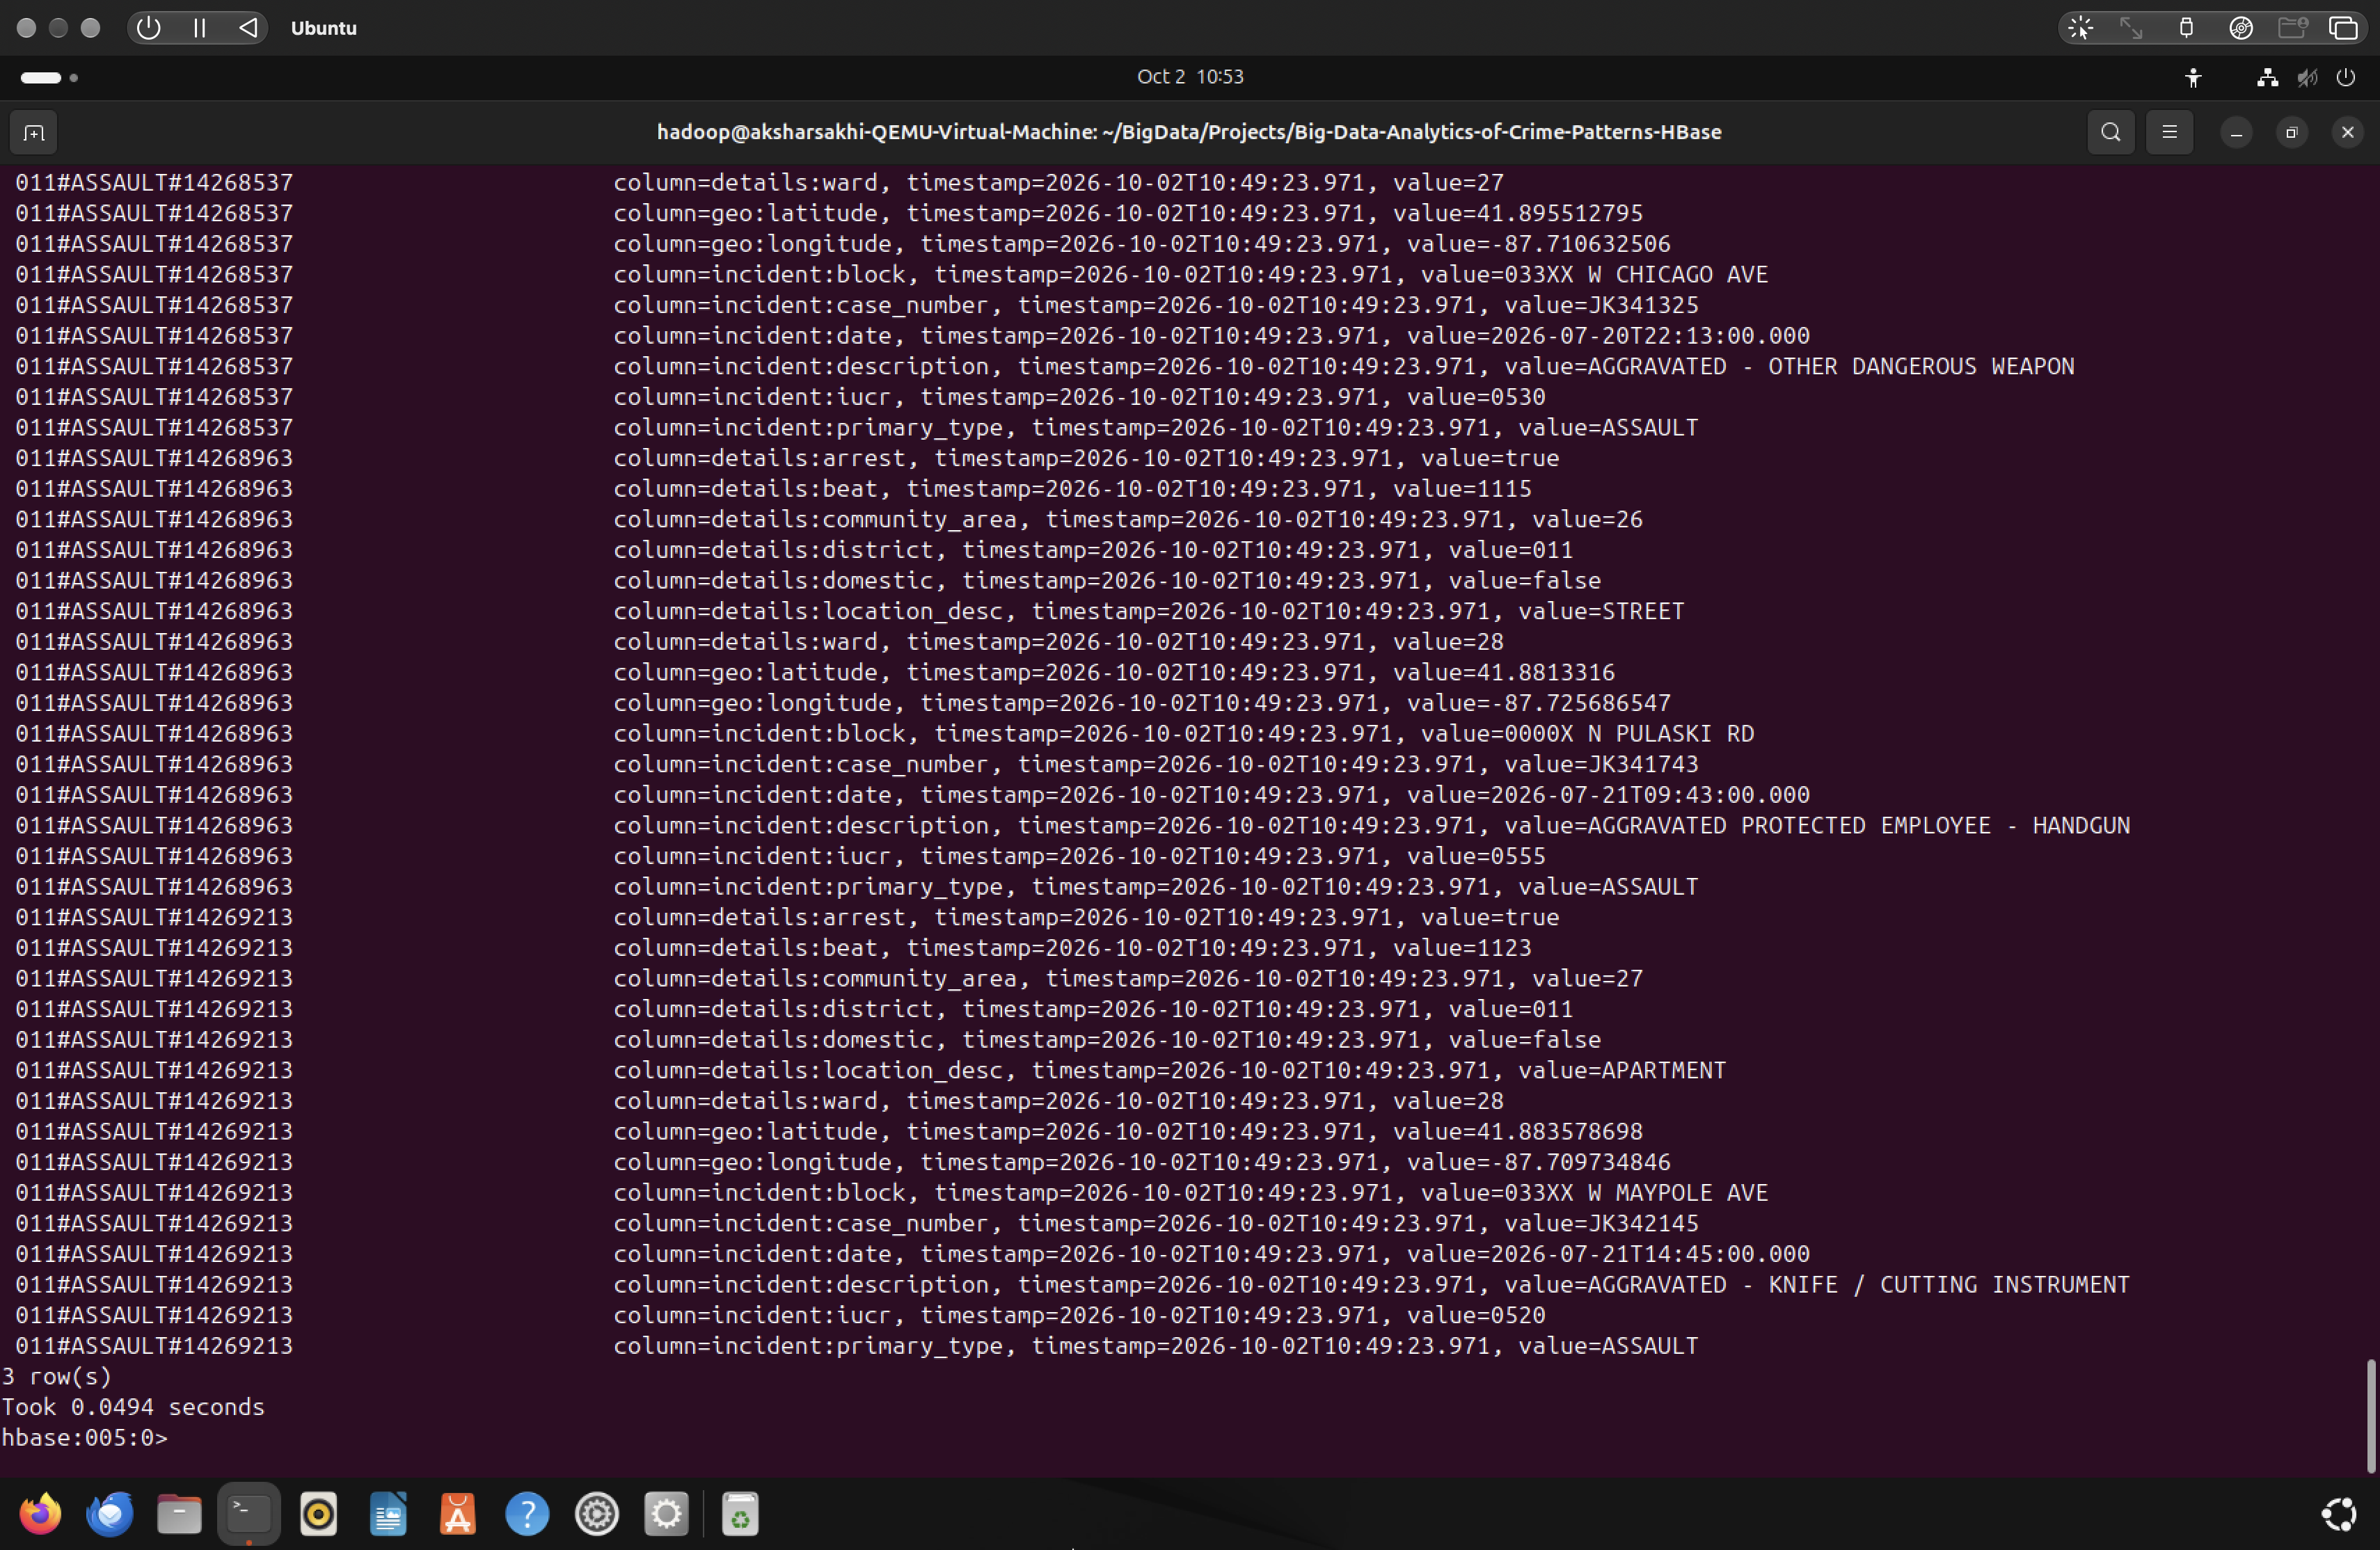
\includegraphics[width=\linewidth,height=3.35cm,keepaspectratio]{images/09_hbase_filter_prefix_011_pt2.png}
        \end{column}
    \end{columns}
    \vspace{0.03cm}
    \begin{itemize}\scriptsize
        \setlength{\itemsep}{1pt}
        \item \textbf{Row-Key Prefix Filtering:} Queries all crimes within District 11 by matching key prefix \texttt{'011\#'}.
        \item \textbf{Fast Region Seeking:} Directly seeks to District 11 blocks, skipping 96\% of irrelevant rows in \textbf{0.0494 seconds}.
        \item \textbf{Operational Impact:} Delivers instant jurisdictional data for district commanders and patrol dispatch.
    \end{itemize}
\end{frame}

% ==========================================================================
% SLIDE 9: HBase Command 4: ValueFilter (Vehicle Crime Investigation)
% ==========================================================================
\begin{frame}[fragile]{Step 4: HBase Shell Command 4 -- \texttt{ValueFilter} (Vehicle Pattern)}
    \noindent\colorbox{LightGray}{\parbox{\dimexpr\linewidth-2\fboxsep\relax}{%
        \fontsize{6.5}{7.5}\selectfont\textbf{Command:} \texttt{scan 'crime\_records', \{FILTER => "ValueFilter(=, 'substring:VEHICLE')", LIMIT => 3\}}%
    }}
    \vskip 0.25cm
    \begin{columns}[T]
        \begin{column}{0.53\textwidth}
            \textbf{\textcolor{NavyBlue}{Live Terminal Execution Proof:}}
            \vspace{0.04cm}
            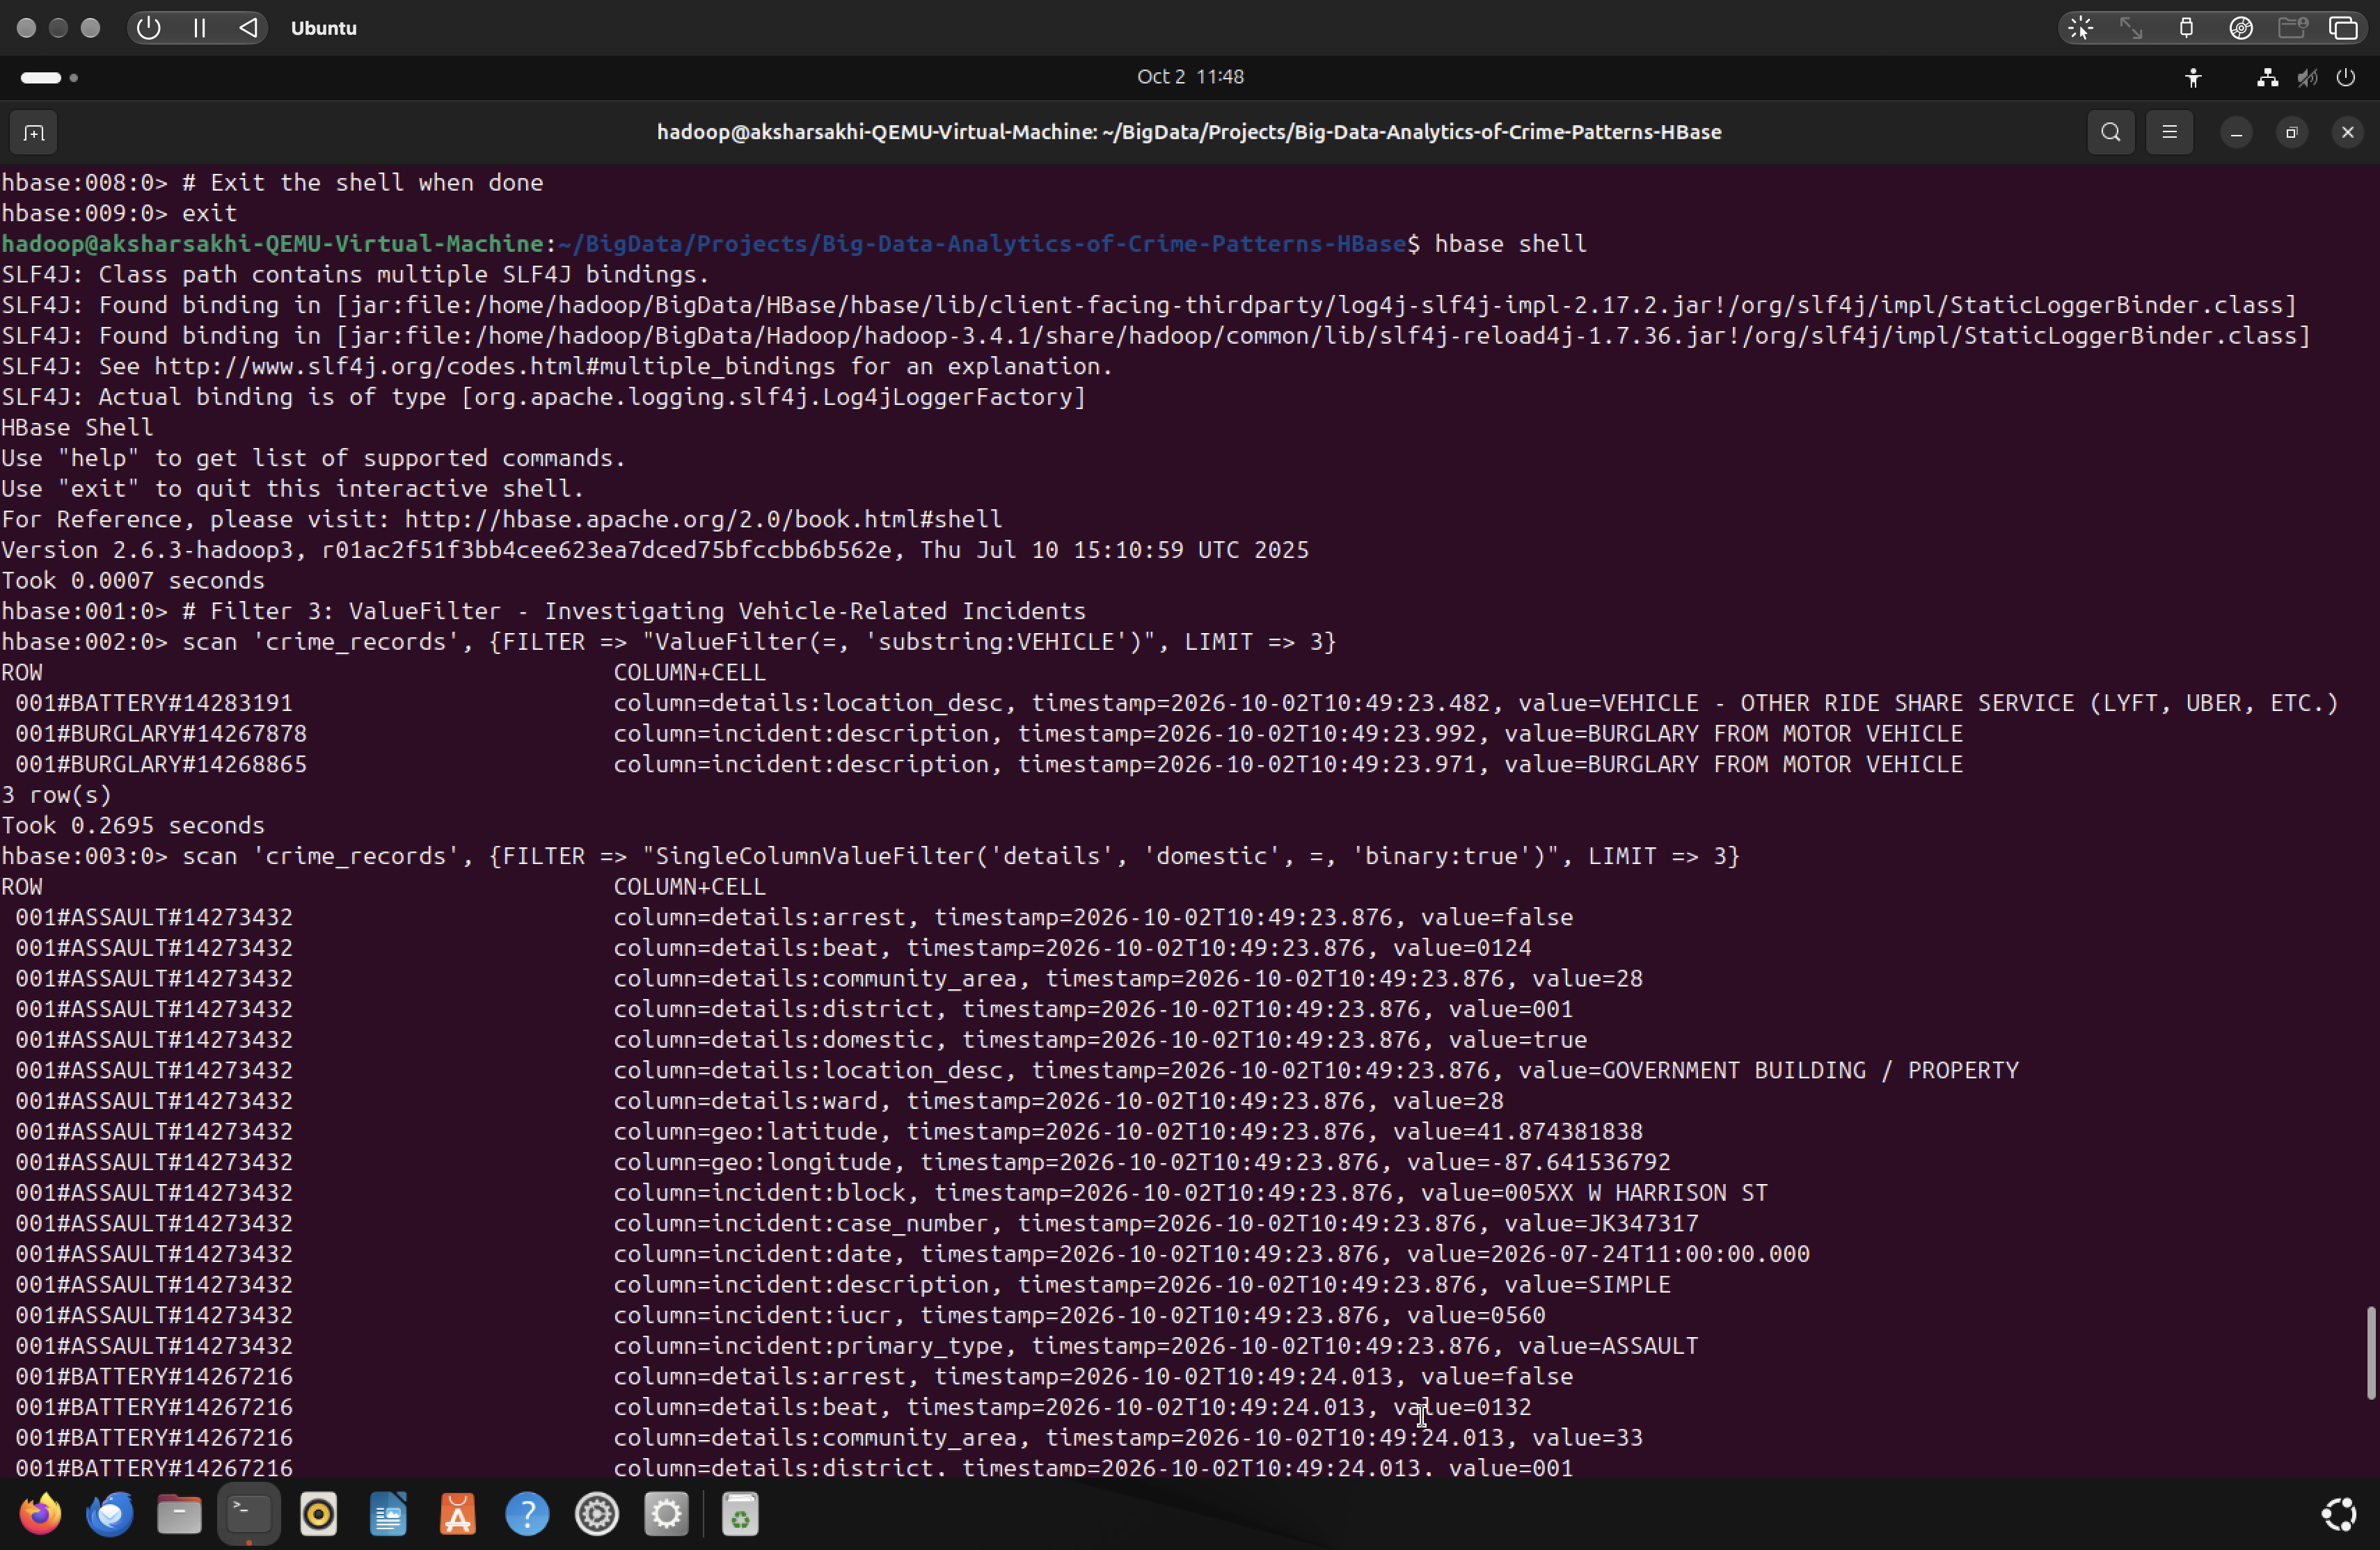
\includegraphics[width=\linewidth,height=4.2cm,keepaspectratio]{images/11_hbase_filter_vehicle_substring.png}
        \end{column}
        \begin{column}{0.45\textwidth}
            \textbf{\textcolor{NavyBlue}{Forensic Value Filtering:}}
            \vspace{0.04cm}
            \begin{itemize}\scriptsize
                \setlength{\itemsep}{2.5pt}
                \item \textbf{Substring Search:} Evaluates cells across all columns and families for keyword \texttt{'VEHICLE'}.
                \item \textbf{Pattern Detection:} Uncovers vehicle thefts, transit incidents, and motor vehicle burglaries in \textbf{0.2695 seconds}.
                \item \textbf{Flexible Querying:} Eliminates the need to know the specific column or exact case identifier beforehand.
                \item \textbf{Investigative Impact:} Enables detectives to identify modus operandi and recurring vehicle-related crimes.
            \end{itemize}
        \end{column}
    \end{columns}
\end{frame}

% ==========================================================================
% SLIDE 10: HBase Command 5: Aggregation Count (COUNT)
% ==========================================================================
\begin{frame}[fragile]{Step 4: HBase Shell Command 5 -- Aggregation Count (\texttt{COUNT})}
    \noindent\colorbox{LightGray}{\parbox{\dimexpr\linewidth-2\fboxsep\relax}{%
        \scriptsize\textbf{Executed Command:} \texttt{count 'crime\_records', INTERVAL => 1000}%
    }}
    \vskip 0.25cm
    \begin{columns}[T]
        \begin{column}{0.53\textwidth}
            \textbf{\textcolor{NavyBlue}{Live Terminal Execution Output:}}
            \vspace{0.04cm}
            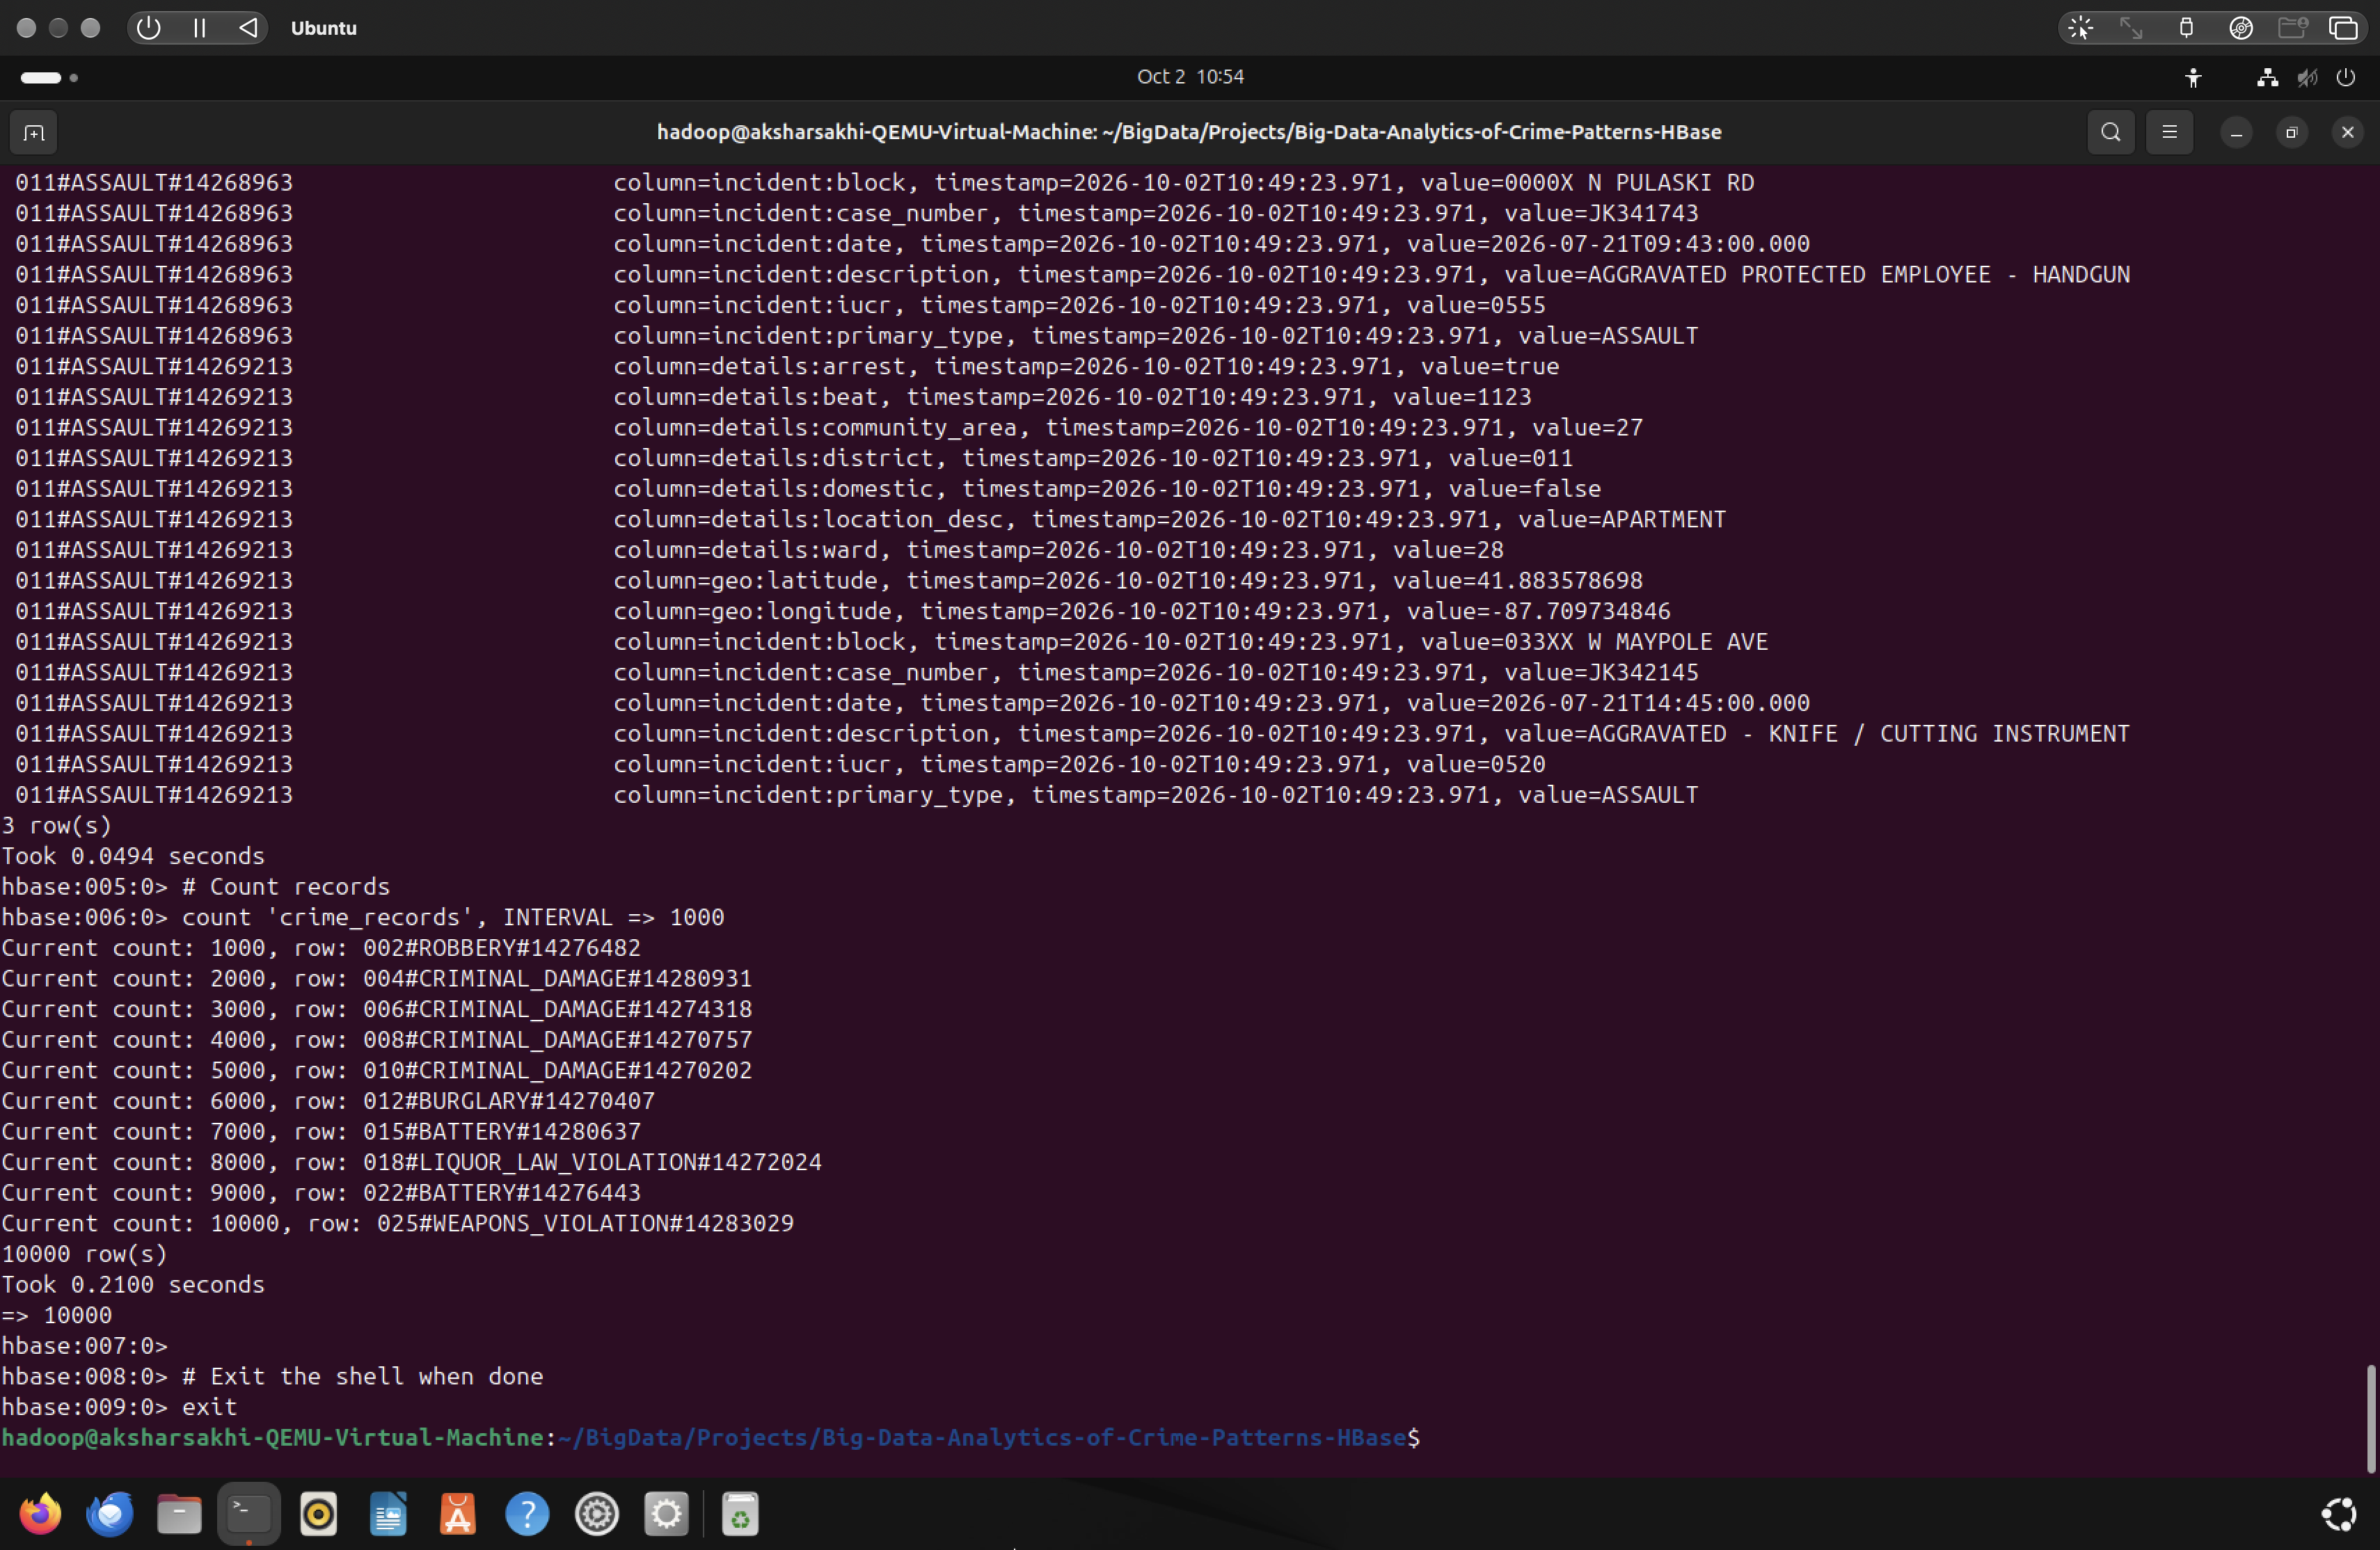
\includegraphics[width=\linewidth,height=4.2cm,keepaspectratio]{images/10_hbase_shell_count_10k_rows.png}
        \end{column}
        \begin{column}{0.45\textwidth}
            \textbf{\textcolor{NavyBlue}{Audit \& Aggregation Analysis:}}
            \vspace{0.04cm}
            \begin{itemize}\scriptsize
                \setlength{\itemsep}{2.5pt}
                \item \textbf{Full Table Audit:} Aggregates and verifies all \textbf{10,000 authentic crime rows} loaded into HBase.
                \item \textbf{Client-Side Caching:} Sets \texttt{INTERVAL => 1000} to stream progress checkpoints every 1,000 records.
                \item \textbf{Sub-Second Scan:} Sequentially scans all 10,000 distributed keys in just \textbf{0.2100 seconds}.
                \item \textbf{Data Integrity:} Confirms 100\% complete ingestion from CSV with zero record drops.
            \end{itemize}
        \end{column}
    \end{columns}
\end{frame}

% ==========================================================================
% SLIDE 11: HBase Command 6: DML Operations (PUT, DELETE, DELETEALL)
% ==========================================================================
\begin{frame}[fragile]{Step 4: HBase Shell Command 6 -- DML (\texttt{PUT}, \texttt{DELETE}, \texttt{DELETEALL})}
    \noindent\colorbox{LightGray}{\parbox{\dimexpr\linewidth-2\fboxsep\relax}{%
        \scriptsize\textbf{Workflow:} Manual \texttt{put} $\rightarrow$ Column \texttt{delete} $\rightarrow$ Row \texttt{deleteall} $\rightarrow$ Verification \texttt{get}%
    }}
    \vskip 0.25cm
    \begin{columns}[T]
        \begin{column}{0.53\textwidth}
            \textbf{\textcolor{NavyBlue}{Live Terminal Execution Proof:}}
            \vspace{0.04cm}
            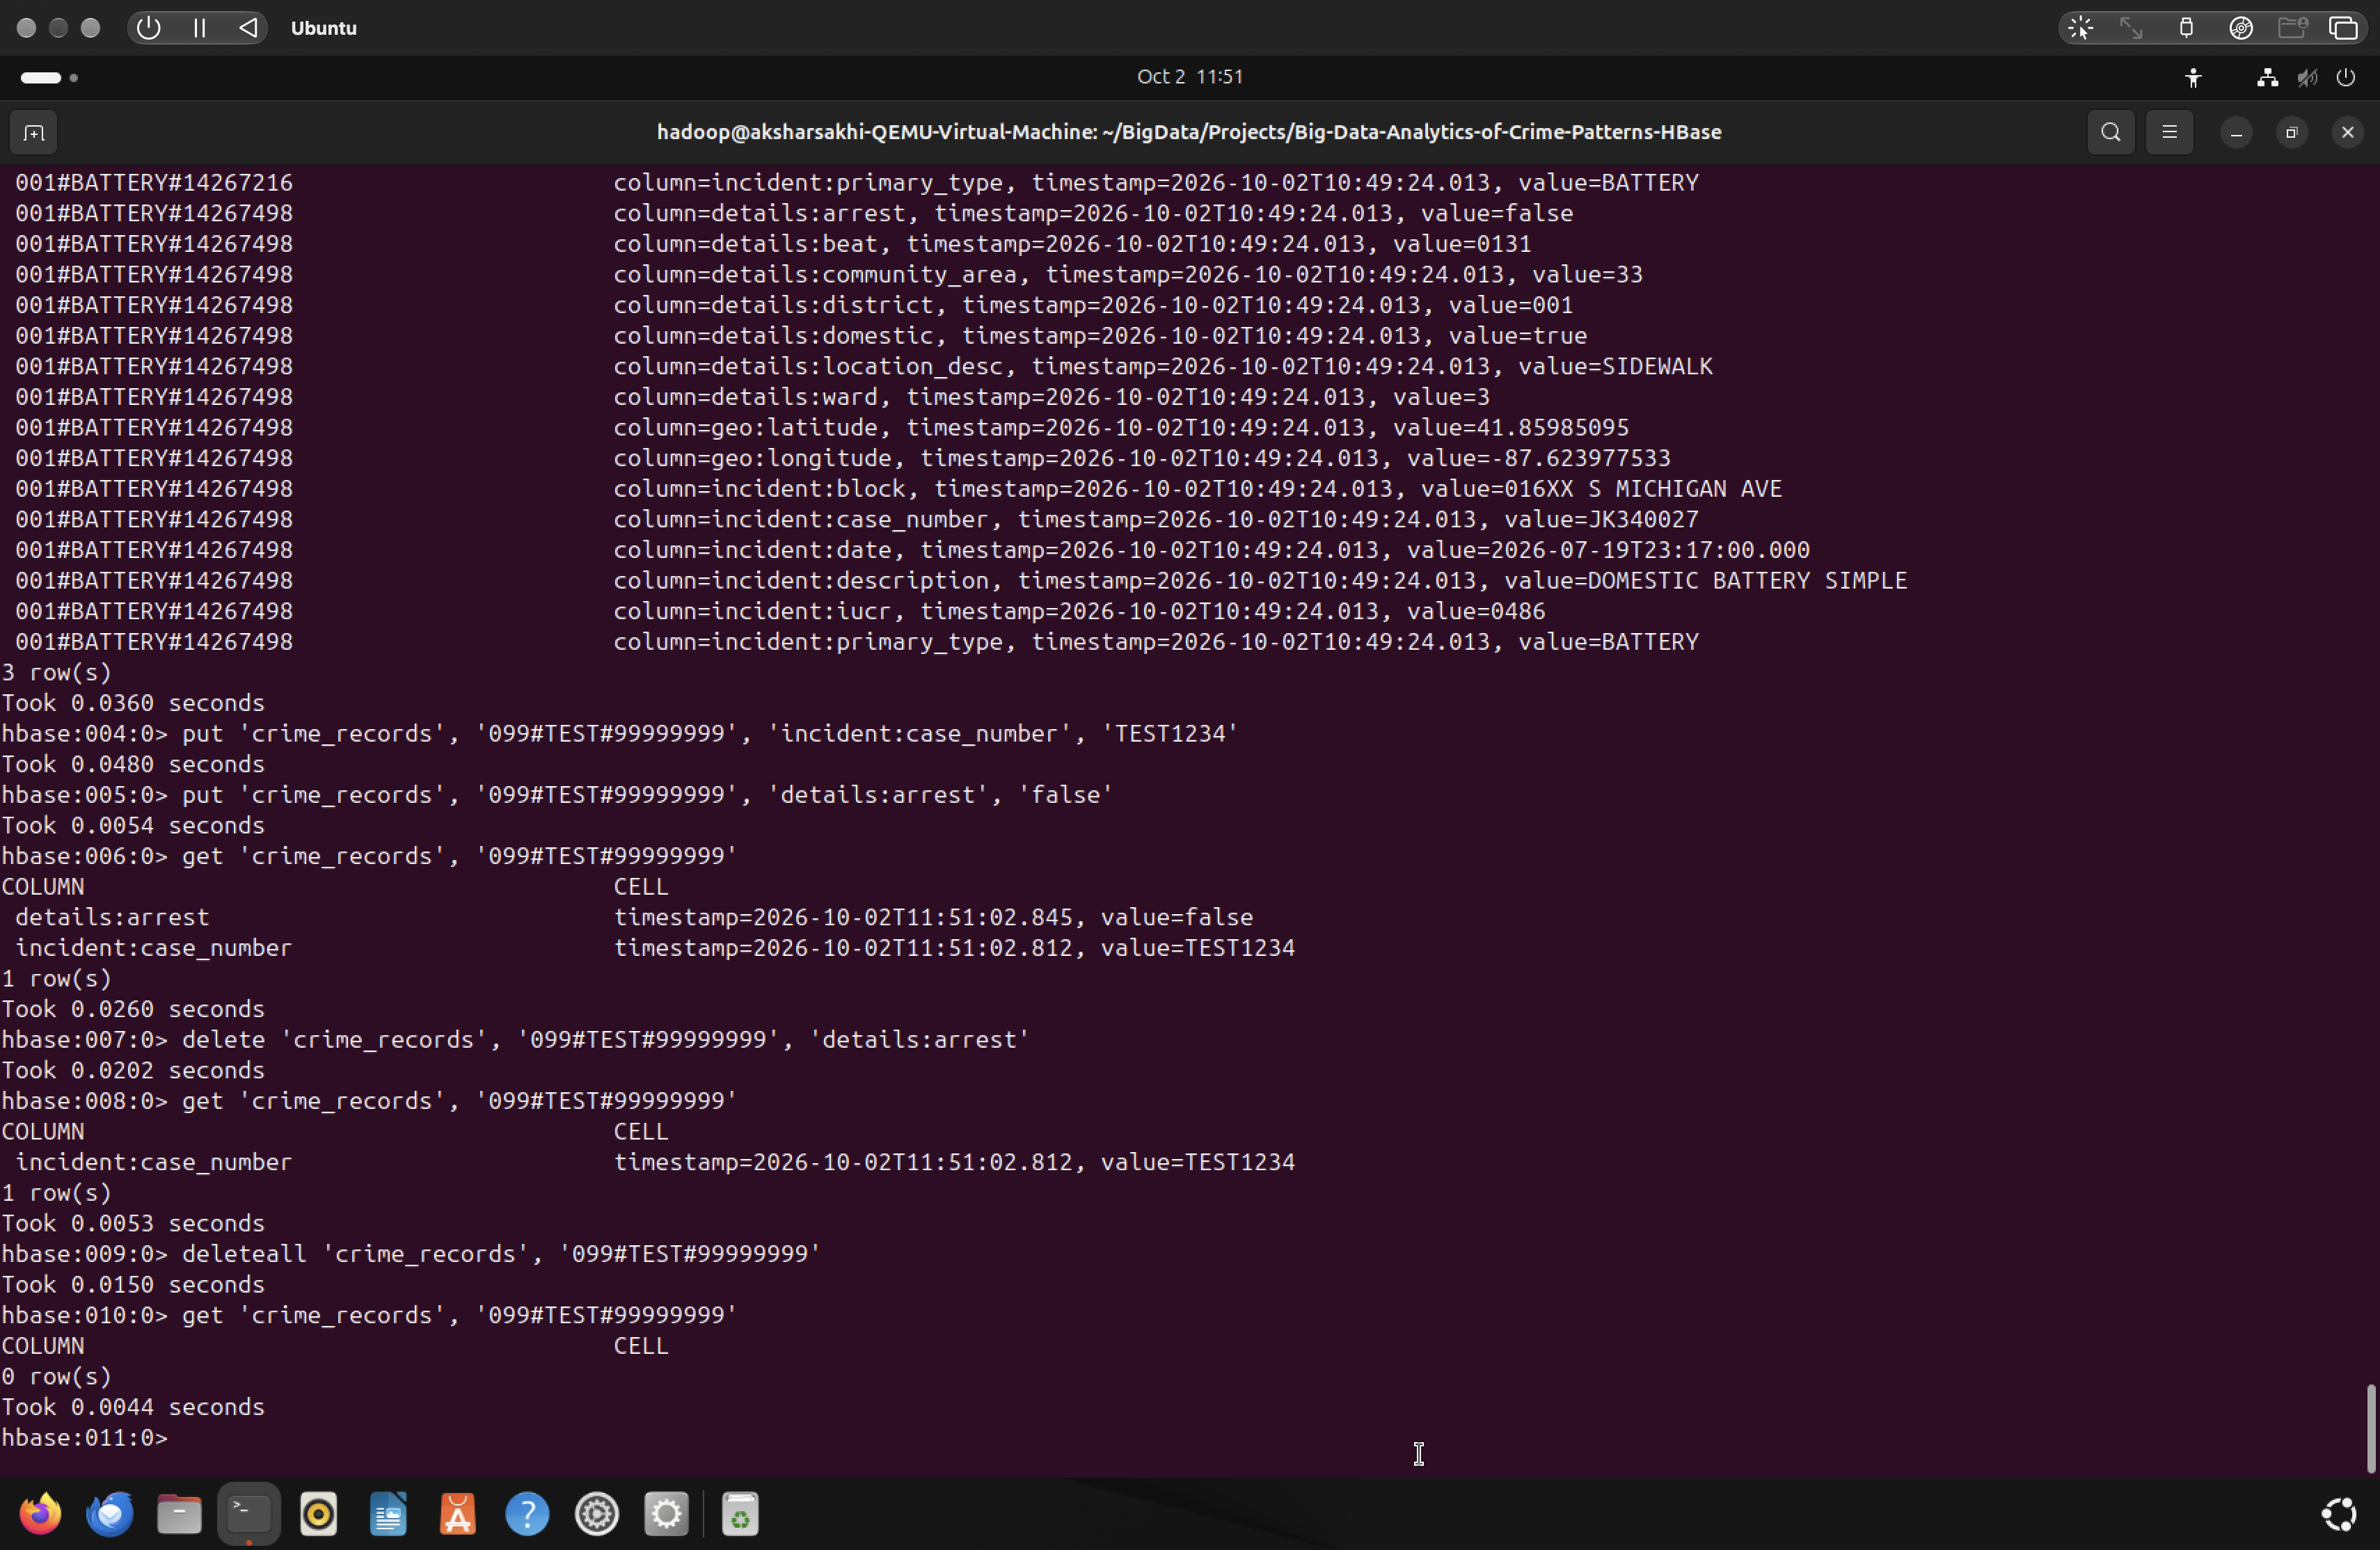
\includegraphics[width=\linewidth,height=4.2cm,keepaspectratio]{images/13_hbase_shell_put_delete_deleteall.png}
        \end{column}
        \begin{column}{0.45\textwidth}
            \textbf{\textcolor{NavyBlue}{Data Modification \& Deletion:}}
            \vspace{0.04cm}
            \begin{itemize}\scriptsize
                \setlength{\itemsep}{2.5pt}
                \item \textbf{Record Insertion (\texttt{put}):} Manually writes test record \texttt{099\#TEST\#99999999} across \texttt{incident} and \texttt{details}.
                \item \textbf{Column Delete (\texttt{delete}):} Drops specific cell \texttt{details:arrest}; verified by \texttt{get} showing only remaining fields.
                \item \textbf{Row Purge (\texttt{deleteall}):} Writes tombstones to expunge the entire row; final \texttt{get} confirms \textbf{0 row(s)} remaining.
                \item \textbf{Lifecycle Verified:} Proves cell-level and row-level ACID mutations and consistency in HBase.
            \end{itemize}
        \end{column}
    \end{columns}
\end{frame}

% ==========================================================================
% SLIDE 12: HBase Java API Implementation & Live Execution
% ==========================================================================
\begin{frame}[fragile]{Step 5: HBase Java API Implementation \& Live Execution}
    \begin{columns}[T]
        \begin{column}{0.48\textwidth}
            \textbf{\textcolor{NavyBlue}{\texttt{HBaseCrimeOperations.java}:}}
            \vspace{0.04cm}
            \begin{lstlisting}[language=Java,basicstyle=\ttfamily\fontsize{4.6}{5.5}\selectfont\color{DarkGray}]
Configuration config = HBaseConfiguration.create();
try (Connection conn = ConnectionFactory.createConnection(config);
     Table table = conn.getTable(TableName.valueOf("crime_records"))) {
  
  // Filtered Scan: Arrest tracking
  Scan scan = new Scan();
  SingleColumnValueFilter filter = new SingleColumnValueFilter(
      Bytes.toBytes("details"), Bytes.toBytes("arrest"),
      CompareOperator.EQUAL, new BinaryComparator(Bytes.toBytes("true")));
  filter.setFilterIfMissing(true);
  scan.setFilter(filter).setLimit(5);

  try (ResultScanner scanner = table.getScanner(scan)) {
    for (Result r : scanner) {
      System.out.println("Match: " + Bytes.toString(r.getRow()));
    }
  }
}
            \end{lstlisting}
            \vspace{0.03cm}
            \noindent\colorbox{LightGray}{\parbox{\dimexpr\linewidth-2\fboxsep\relax}{%
                \tiny\textbf{Pipeline:} Admin check $\rightarrow$ Put $\rightarrow$ Get $\rightarrow$ Filter Scan $\rightarrow$ Delete \& Verify.%
            }}
        \end{column}
        \begin{column}{0.50\textwidth}
            \textbf{\textcolor{NavyBlue}{Live Execution Proof (\texttt{run\_java\_api.sh}):}}
            \vspace{0.04cm}
            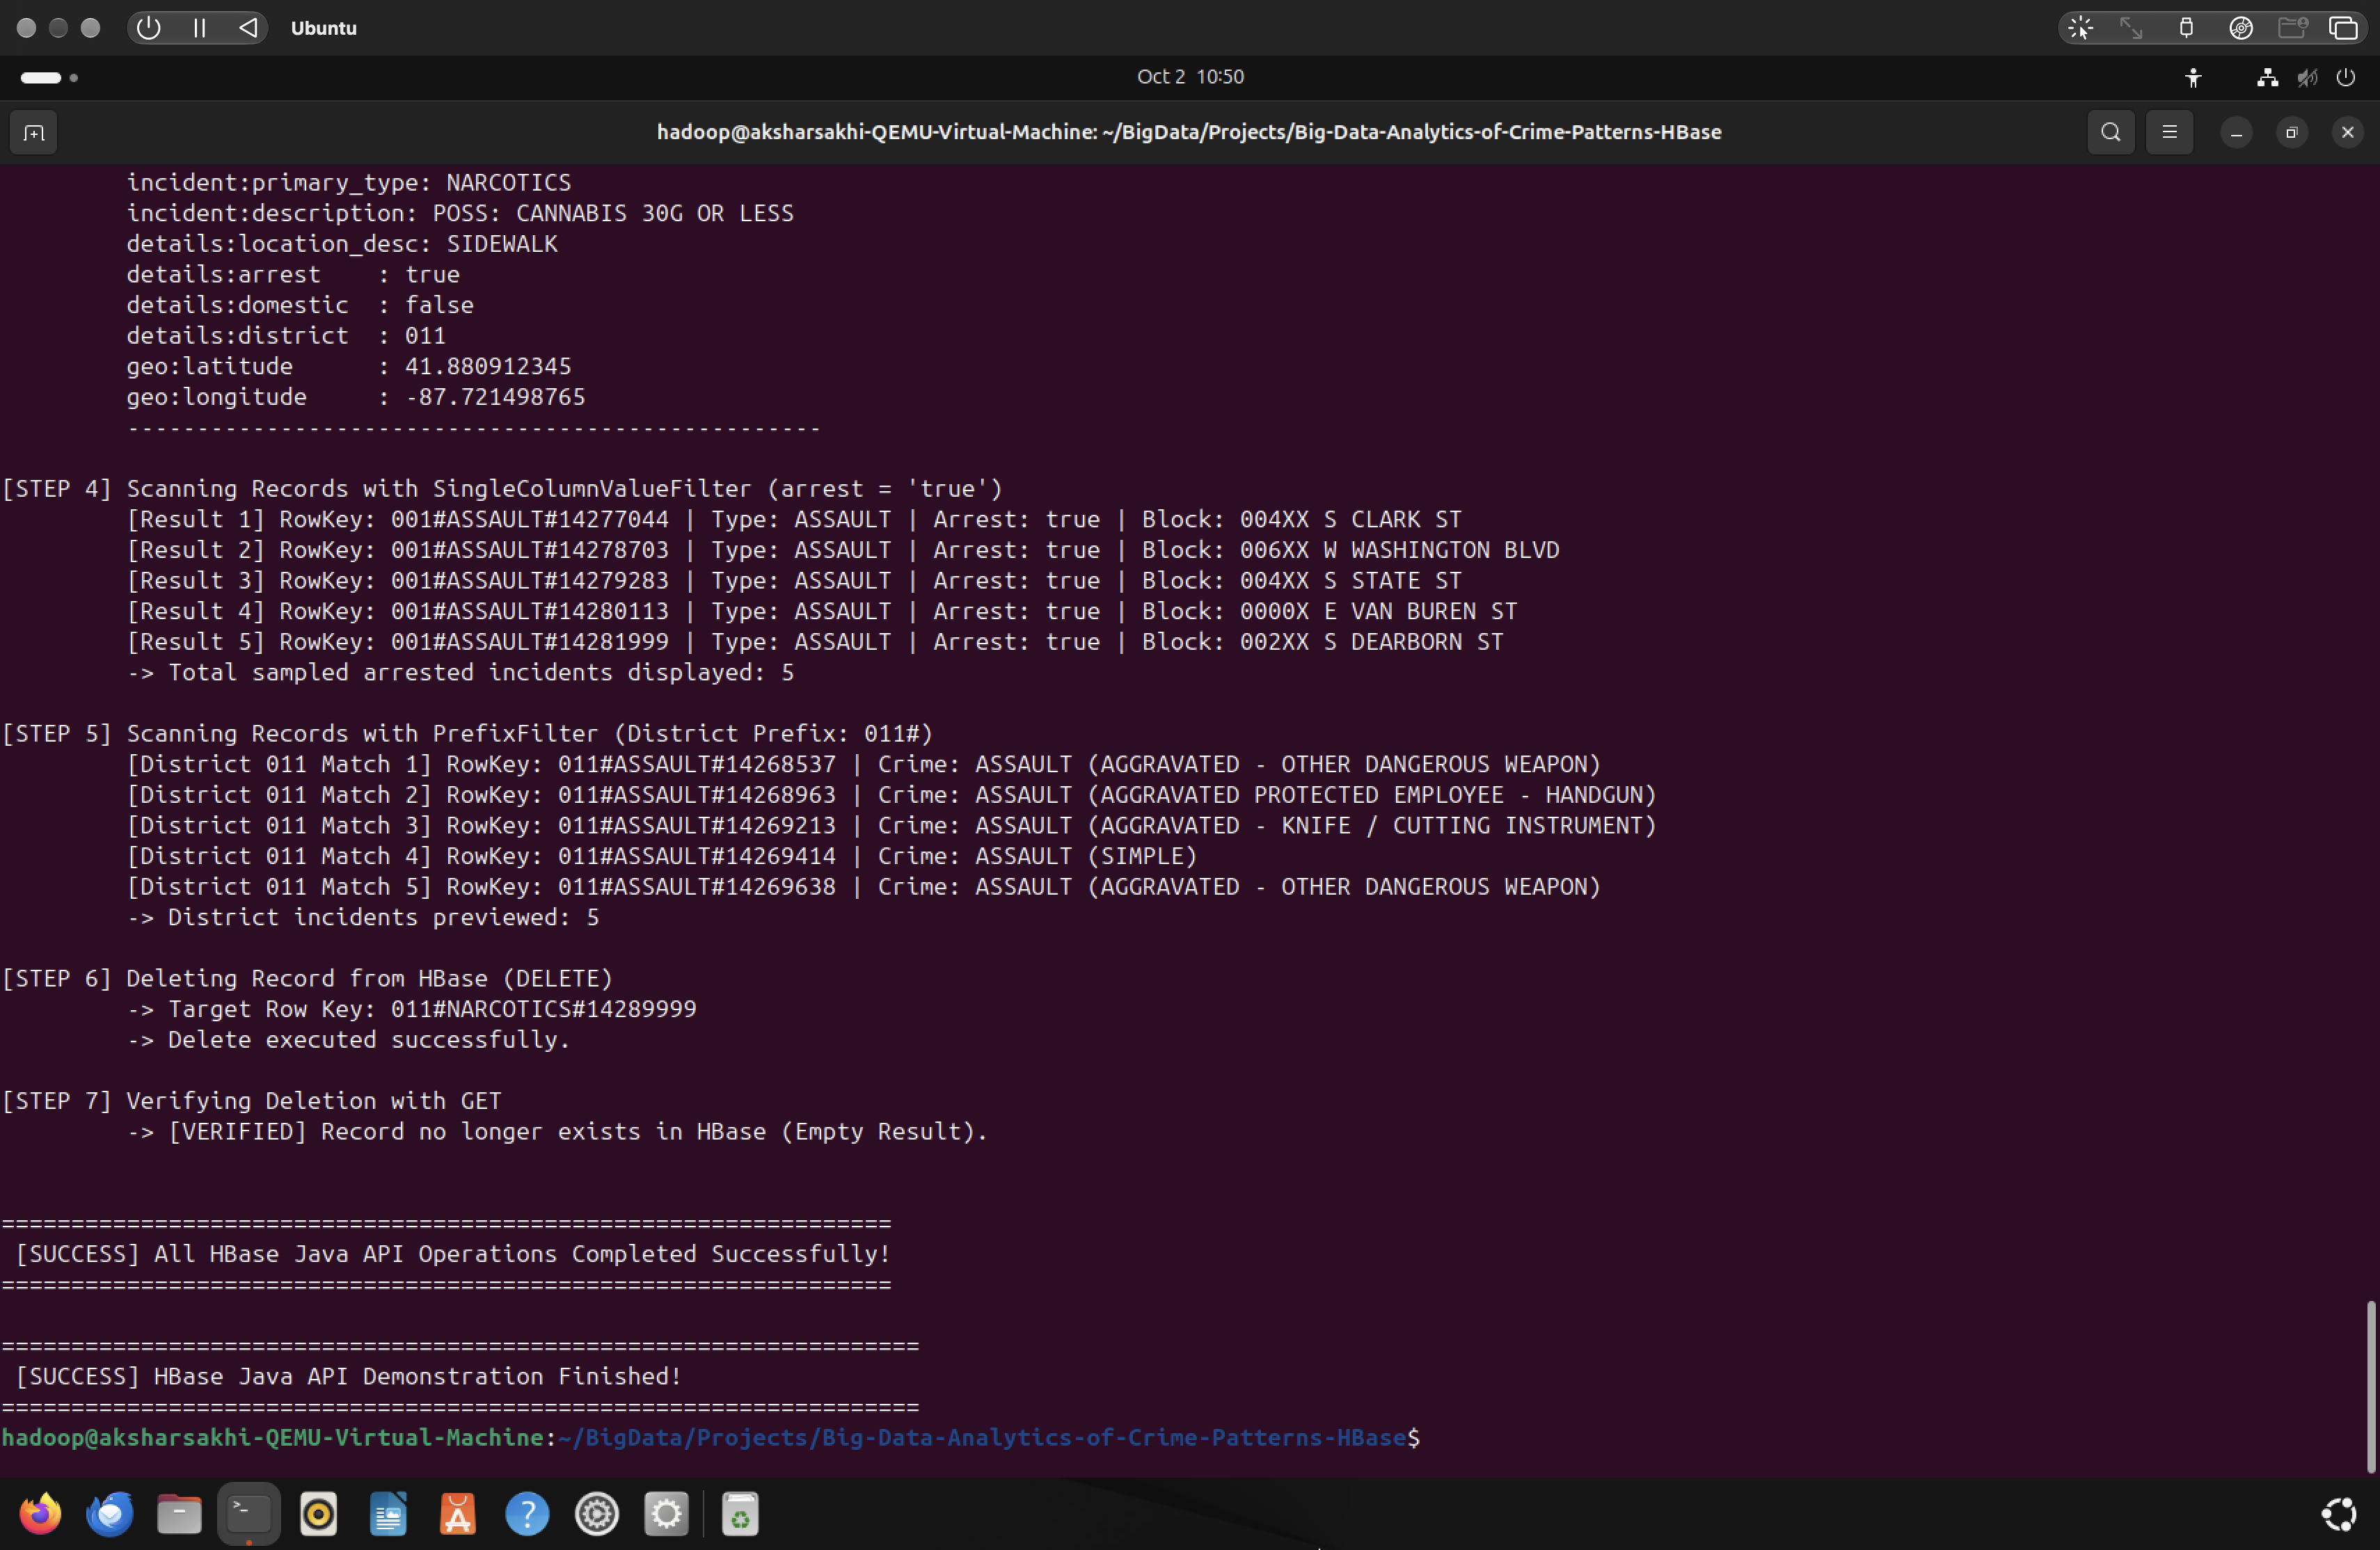
\includegraphics[width=\linewidth,height=3.4cm,keepaspectratio]{images/03_java_api_execution.png}
            \vspace{0.03cm}
            \begin{itemize}\tiny
                \setlength{\itemsep}{1.5pt}
                \item \textbf{Programmatic API:} Connects via \texttt{ConnectionFactory} executing the full CRUD pipeline in Java.
                \item \textbf{Filtered Scanner:} Programmatically tracks arrests and streams row keys directly from HBase.
                \item \textbf{Live Verification:} Terminal log confirms \textbf{[SUCCESS]} with zero connection or RPC errors.
            \end{itemize}
        \end{column}
    \end{columns}
\end{frame}


% ==========================================================================
% SLIDE 13: Conclusion & Evaluation Rubric Compliance
% ==========================================================================
\begin{frame}{Conclusion \& Evaluation Rubric Compliance}
    \begin{columns}[T]
        \begin{column}{0.44\textwidth}
            \textbf{\textcolor{NavyBlue}{Project Review 2 Summary:}}
            \begin{itemize}\scriptsize
                \setlength{\itemsep}{2pt}
                \item Successfully ported crime analytics from batch OLAP (Review 1) to real-time NoSQL serving on \textbf{Apache HBase}.
                \item Balanced load across RegionServers using composite key (\texttt{District\#CrimeType\#ID}).
                \item Demonstrated comprehensive HBase Shell commands (\texttt{describe}, \texttt{get}, filters, \texttt{count}, \texttt{delete}) with sub-second response times.
                \item Implemented native Java API client (\texttt{HBaseCrimeOperations.java}) executing full lifecycle operations.
                \item Verified on 10,000 authentic City of Chicago crime records.
            \end{itemize}
            \vspace{0.1cm}
            \centering
            \colorbox{LightGray}{\textbf{\scriptsize\textcolor{AmritaMaroon}{Thank You! Questions \& Live Demonstration.}}}
        \end{column}
        \begin{column}{0.54\textwidth}
            \vspace{-0.15cm}
            {\fontsize{5.8}{7.2}\selectfont
            \begin{table}
                \centering
                \setlength{\tabcolsep}{3.5pt}
                \renewcommand{\arraystretch}{1.12}
                \begin{tabular}{>{\raggedright\arraybackslash}p{2.55cm}cp{3.45cm}}
                    \toprule
                    \textbf{Evaluation Criteria} & \textbf{Marks} & \textbf{Evidence} \\
                    \midrule
                    Real-world problem \& dataset selection & 1 & Chicago Crimes authentic dataset (10K+ records, 22 attributes) \\
                    HBase table design \& schema & 1 & Composite row key (\texttt{Dist\#Type\#ID}); 3 column families \\
                    HBase Shell implementation & 2 & \texttt{create}, \texttt{describe}, \texttt{put}, \texttt{get}, \texttt{scan}, \texttt{count}, \texttt{delete}, \texttt{deleteall} verified \\
                    HBase Filters \& analytical queries & 4 & $\ge 3$ filters: \texttt{SingleColumnValueFilter}, \texttt{PrefixFilter}, \texttt{ValueFilter} \\
                    Java API implementation & 2 & \texttt{HBaseCrimeOps.java}: Admin, Put, Get, Filter Scan, Delete \\
                    \midrule
                    \multicolumn{3}{c}{\textbf{All rubric criteria fully satisfied}} \\
                    \bottomrule
                \end{tabular}
            \end{table}
            }
        \end{column}
    \end{columns}
\end{frame}

\end{document}
